% ============================================================
% main_full.tex
% Topic: RL + Avellaneda-Stoikov (AS) + Limit Order Book (LOB) HFT Market Making
% Compile:
%   pdflatex main_full.tex
%   biber main_full
%   pdflatex main_full.tex
%   pdflatex main_full.tex
% ============================================================

\documentclass[11pt]{article}

% ----------------------------
% Packages
% ----------------------------
\usepackage[a4paper,margin=1in]{geometry}
\usepackage{setspace}
\usepackage{microtype}
\usepackage{amsmath,amssymb,amsthm}
\usepackage{booktabs}
\usepackage{graphicx}
\usepackage{caption}
\usepackage{subcaption}
\usepackage{hyperref}
\usepackage{xcolor}
\usepackage{enumitem}
\usepackage{algorithm}
\usepackage{algorithmic}
\usepackage{float}
\usepackage{array}
\usepackage{longtable}
\usepackage{multirow}
\usepackage{mathtools}
\usepackage{siunitx}
\usepackage{makecell}

\hypersetup{
  colorlinks=true,
  linkcolor=blue,
  citecolor=blue,
  urlcolor=blue
}

\onehalfspacing

% ----------------------------
% BibLaTeX
% ----------------------------
\usepackage[
  backend=biber,
  style=apa,
  doi=true,
  url=false,
  isbn=false,
  eprint=false
]{biblatex}

\begin{filecontents*}{references.bib}

@article{ho1981dealer,
  title   = {Optimal dealer pricing under transactions and return uncertainty},
  author  = {Ho, Thomas and Stoll, Hans R.},
  journal = {Journal of Financial Economics},
  volume  = {9},
  number  = {1},
  pages   = {47--73},
  year    = {1981},
  doi     = {10.1016/0304-405X(81)90020-9}
}

@book{ohara1995microstructure,
  title     = {Market Microstructure Theory},
  author    = {O'Hara, Maureen},
  publisher = {Blackwell},
  year      = {1995}
}

@article{avellaneda2008hftlob,
  title   = {High-frequency trading in a limit order book},
  author  = {Avellaneda, Marco and Stoikov, Sasha},
  journal = {Quantitative Finance},
  volume  = {8},
  number  = {3},
  pages   = {217--224},
  year    = {2008},
  doi     = {10.1080/14697680701381228}
}

@article{gueant2013inventory,
  title   = {Dealing with the inventory risk: a solution to the market making problem},
  author  = {Gu{\'e}ant, Olivier and Lehalle, Charles-Albert and Fernandez-Tapia, Joaquin},
  journal = {Mathematics and Financial Economics},
  volume  = {7},
  number  = {4},
  pages   = {477--507},
  year    = {2013},
  doi     = {10.1007/s11579-012-0087-0}
}

@article{cont2013markovlob,
  title   = {Price dynamics in a Markovian limit order market},
  author  = {Cont, Rama and de Larrard, Adrien},
  journal = {SIAM Journal on Financial Mathematics},
  volume  = {4},
  number  = {1},
  pages   = {1--25},
  year    = {2013},
  doi     = {10.1137/110856605}
}

@book{cartea2015ahft,
  title     = {Algorithmic and High-Frequency Trading},
  author    = {Cartea, {\'A}lvaro and Jaimungal, Sebastian and Penalva, Jos{\'e}},
  publisher = {Cambridge University Press},
  year      = {2015}
}

@article{cartea2015execution,
  title   = {Optimal execution with limit and market orders},
  author  = {Cartea, {\'A}lvaro and Jaimungal, Sebastian},
  journal = {Quantitative Finance},
  volume  = {15},
  number  = {8},
  pages   = {1279--1291},
  year    = {2015},
  doi     = {10.1080/14697688.2015.1032543}
}

@inproceedings{spooner2018mmrl,
  title     = {Market Making via Reinforcement Learning},
  author    = {Spooner, Thomas and Fearnley, John and Savani, Rahul and Koukorinis, Andreas},
  booktitle = {Proceedings of the 17th International Conference on Autonomous Agents and MultiAgent Systems (AAMAS)},
  pages     = {434--442},
  year      = {2018}
}

@article{gasperov2021rlmm,
  title   = {Reinforcement Learning Approaches to Optimal Market Making},
  author  = {Ga{\v s}perov, Bruno and Begu{\v s}i{\'c}, Stjepan and Posedel {\v S}imovi{\'c}, Petra and Kostanj{\v c}ar, Zvonko},
  journal = {Mathematics},
  volume  = {9},
  number  = {21},
  pages   = {2689},
  year    = {2021},
  doi     = {10.3390/math9212689}
}

@misc{gasperov2022hawkesmm,
  title        = {Deep Reinforcement Learning for Market Making Under a Hawkes Process-Based Limit Order Book Model},
  author       = {Ga{\v s}perov, Bruno and Kostanj{\v c}ar, Zvonko},
  year         = {2022},
  doi          = {10.48550/arXiv.2207.09951}
}

@article{lalor2025nonmarkov,
  title   = {Deep Reinforcement Learning in Non-Markov Market-Making},
  author  = {Lalor, Luca and Swishchuk, Anatoliy},
  journal = {Risks},
  volume  = {13},
  number  = {3},
  pages   = {40},
  year    = {2025},
  doi     = {10.3390/risks13030040}
}

@misc{sadighian2019crypto,
  title        = {Deep Reinforcement Learning in Cryptocurrency Market Making},
  author       = {Sadighian, Jonathan},
  year         = {2019},
  doi          = {10.48550/arXiv.1911.08647}
}

@article{falces2022asrl,
  title   = {A reinforcement learning approach to improve the performance of the Avellaneda--Stoikov market-making algorithm},
  author  = {Falces Mar{\'i}n, Javier and D{\'i}az Pardo de Vera, David and Lopez Gonzalo, Eduardo},
  journal = {PLOS ONE},
  volume  = {17},
  number  = {12},
  pages   = {e0277042},
  year    = {2022},
  doi     = {10.1371/journal.pone.0277042}
}

@misc{byrd2019abides,
  title        = {ABIDES: Towards High-Fidelity Market Simulation for AI Research},
  author       = {Byrd, David and Hybinette, Maria and Balch, Tucker Hybinette},
  year         = {2019},
  doi          = {10.48550/arXiv.1904.12066}
}

@misc{amrouni2021abidesgym,
  title        = {ABIDES-Gym: Gym Environments for Multi-Agent Discrete Event Simulation and Application to Financial Markets},
  author       = {Amrouni, Selim and Moulin, Aymeric and Vann, Jared and Vyetrenko, Svitlana and Balch, Tucker and Veloso, Manuela},
  year         = {2021},
  doi          = {10.48550/arXiv.2110.14771}
}

@misc{karpe2020marl,
  title        = {Multi-Agent Reinforcement Learning in a Realistic Limit Order Book Market Simulation},
  author       = {Karpe, Micha{\"e}l and Fang, Jin and Ma, Zhongyao and Wang, Chen},
  year         = {2020},
  doi          = {10.48550/arXiv.2006.05574}
}

@inproceedings{jerome2023mbtgym,
  title     = {Mbt-gym: Reinforcement learning for model-based limit order book trading},
  author    = {Jerome, Joseph and S{\'a}nchez-Betancourt, Leandro and Savani, Rahul and Herdegen, Martin},
  booktitle = {Proceedings of the 4th ACM International Conference on AI in Finance (ICAIF '23)},
  pages     = {619--627},
  year      = {2023},
  doi       = {10.1145/3604237.3626873}
}

@inproceedings{frey2023jaxlob_acm,
  title     = {JAX-LOB: a GPU-Accelerated limit order book simulator to unlock large scale reinforcement learning for trading},
  author    = {Frey, Sascha and Li, Kang and Nagy, Peer and Sapora, Silvia and Lu, Chris and Zohren, Stefan and Foerster, Jakob and Calinescu, Anisoara},
  booktitle = {Proceedings of the 4th ACM International Conference on AI in Finance (ICAIF '23)},
  pages     = {583--591},
  year      = {2023},
  doi       = {10.1145/3604237.3626880}
}

@misc{frey2023jaxlob_arxiv,
  title        = {JAX-LOB: A GPU-Accelerated limit order book simulator to unlock large scale reinforcement learning for trading},
  author       = {Frey, Sascha and Li, Kang and Nagy, Peer and Sapora, Silvia and Lu, Chris and Zohren, Stefan and Foerster, Jakob and Calinescu, Anisoara},
  year         = {2023},
  doi          = {10.48550/arXiv.2308.13289}
}

@article{ntakaris2018fi2010,
  title   = {Benchmark dataset for mid-price forecasting of limit order book data with machine learning methods},
  author  = {Ntakaris, Adamantios and Magris, Martin and Kanniainen, Juho and Gabbouj, Moncef and Iosifidis, Alexandros},
  journal = {Journal of Forecasting},
  volume  = {37},
  number  = {8},
  pages   = {852--866},
  year    = {2018},
  doi     = {10.1002/for.2543}
}

@article{zhang2019deeplob,
  title   = {DeepLOB: Deep Convolutional Neural Networks for Limit Order Books},
  author  = {Zhang, Zihao and Zohren, Stefan and Roberts, Stephen J.},
  journal = {IEEE Transactions on Signal Processing},
  volume  = {67},
  number  = {11},
  pages   = {3001--3012},
  year    = {2019},
  doi     = {10.1109/TSP.2019.2907260}
}

@misc{lobsterdata,
  title        = {LOBSTER: High-frequency limit order book data},
  howpublished = {\url{https://lobsterdata.com/}},
  note         = {Accessed 2026-02-16}
}

@misc{lobbench2025,
  title        = {LOB-Bench: Benchmarking Generative AI for Finance -- an Application to Limit Order Book Data},
  author       = {Nagy, Peer and Frey, Sascha and Li, Kang and Sarkar, Bidipta and Vyetrenko, Svitlana and Zohren, Stefan and Calinescu, Anisoara and Foerster, Jakob},
  year         = {2025},
  doi          = {10.48550/arXiv.2502.09172}
}

@article{schulman2017ppo,
  title        = {Proximal Policy Optimization Algorithms},
  author       = {Schulman, John and Wolski, Filip and Dhariwal, Prafulla and Radford, Alec and Klimov, Oleg},
  journal      = {arXiv preprint arXiv:1707.06347},
  year         = {2017},
  doi          = {10.48550/arXiv.1707.06347}
}

@article{glosten1985bid,
  title   = {Bid, ask and transaction prices in a specialist market with heterogeneously informed traders},
  author  = {Glosten, Lawrence R. and Milgrom, Paul R.},
  journal = {Journal of Financial Economics},
  volume  = {14},
  number  = {1},
  pages   = {71--100},
  year    = {1985},
  doi     = {10.1016/0304-405X(85)90044-3}
}

@article{kyle1985continuous,
  title   = {Continuous Auctions and Insider Trading},
  author  = {Kyle, Albert S.},
  journal = {Econometrica},
  volume  = {53},
  number  = {6},
  pages   = {1315--1335},
  year    = {1985},
  doi     = {10.2307/1913210}
}

@article{hendershott2011does,
  title   = {Does Algorithmic Trading Improve Liquidity?},
  author  = {Hendershott, Terrence and Jones, Charles M. and Menkveld, Albert J.},
  journal = {Journal of Finance},
  volume  = {66},
  number  = {1},
  pages   = {1--33},
  year    = {2011},
  doi     = {10.1111/j.1540-6261.2010.01624.x}
}

@article{menkveld2013high,
  title   = {High frequency trading and the new market makers},
  author  = {Menkveld, Albert J.},
  journal = {Journal of Financial Markets},
  volume  = {16},
  number  = {4},
  pages   = {712--740},
  year    = {2013},
  doi     = {10.1016/j.finmar.2013.06.006}
}

@article{cont2010stochastic,
  title   = {A stochastic model for order book dynamics},
  author  = {Cont, Rama and Stoikov, Sasha and Talreja, Rishi},
  journal = {Operations Research},
  volume  = {58},
  number  = {3},
  pages   = {549--563},
  year    = {2010},
  doi     = {10.1287/opre.1090.0780}
}

@article{guilbaud2013optimal,
  title   = {Optimal high-frequency trading with limit and market orders},
  author  = {Guilbaud, Fabien and Pham, Huy{\^e}n},
  journal = {Quantitative Finance},
  volume  = {13},
  number  = {1},
  pages   = {79--94},
  year    = {2013},
  doi     = {10.1080/14697688.2012.708779}
}

@article{lehalle2019incorporating,
  title   = {Incorporating signals into optimal trading},
  author  = {Lehalle, Charles-Albert and Neuman, Eyal},
  journal = {Finance and Stochastics},
  volume  = {23},
  number  = {2},
  pages   = {275--311},
  year    = {2019},
  doi     = {10.1007/s00780-019-00382-7}
}

@article{almgren2001optimal,
  title   = {Optimal execution of portfolio transactions},
  author  = {Almgren, Robert and Chriss, Neil},
  journal = {Journal of Risk},
  volume  = {3},
  number  = {2},
  pages   = {5--39},
  year    = {2001},
  doi     = {10.21314/JOR.2001.041}
}

@article{stoikov2009option,
  title   = {Option market making under inventory risk},
  author  = {Stoikov, Sasha and Sa{\u{g}}lam, Mehmet},
  journal = {Review of Derivatives Research},
  volume  = {12},
  number  = {1},
  pages   = {55--79},
  year    = {2009},
  doi     = {10.1007/s11147-009-9029-2}
}

@article{altschuler2024multi,
  title   = {Multi-asset market making with inventory constraints and market impact},
  author  = {Altschuler, Dylan and Balata, Antoine and El Aoun, Marouane and Laruelle, Sophie and Lehalle, Charles-Albert},
  journal = {SIAM Journal on Financial Mathematics},
  volume  = {15},
  number  = {1},
  pages   = {160--195},
  year    = {2024},
  doi     = {10.1137/23M1559313}
}

@book{bouchaud2018trades,
  title     = {Trades, Quotes and Prices: Financial Markets Under the Microscope},
  author    = {Bouchaud, Jean-Philippe and Bonart, Julius and Donier, Jonathan and Gould, Martin},
  publisher = {Cambridge University Press},
  year      = {2018},
  doi       = {10.1017/9781316659335}
}

\end{filecontents*}

\addbibresource{references.bib}

% ----------------------------
% Math commands and theorem envs
% ----------------------------
\newcommand{\E}{\mathbb{E}}
\newcommand{\Var}{\mathrm{Var}}
\newcommand{\Cov}{\mathrm{Cov}}
\newcommand{\dd}{\,\mathrm{d}}
\newcommand{\PnL}{\mathrm{PnL}}
\newcommand{\TC}{\mathrm{TC}}
\newcommand{\LOB}{\mathrm{LOB}}
\newcommand{\KL}{\mathrm{KL}}
\newcommand{\CVaR}{\mathrm{CVaR}}

\newtheorem{definition}{Definition}
\newtheorem{assumption}{Assumption}
\newtheorem{proposition}{Proposition}

% ----------------------------
% Title
% ----------------------------
\title{\textbf{Hybrid Reinforcement Learning with an Avellaneda--Stoikov Backbone\\
for Order-Book-Aware High-Frequency Market Making\\
under Non-Stationary Microstructure}}
\author{
  Haoyu Wang \\
  \small University of Auckland \\
  \small \texttt{haoyu.wang@auckland.ac.nz}
}
\date{\today}

\begin{document}
\maketitle

% ============================================================
\begin{abstract}
We develop a structured reinforcement learning (RL) framework for
high-frequency market making in electronic limit order books (LOBs) by
combining the classical Avellaneda--Stoikov (AS) analytical quoting
backbone with a data-driven residual controller trained via Proximal
Policy Optimisation (PPO).
The AS component provides a low-dimensional, interpretable policy class
that encodes the fundamental spread--inventory trade-off derived from
stochastic control theory \parencite{avellaneda2008hftlob,gueant2013inventory},
while the RL residual adapts quoting to non-stationary order flow,
discrete ticks, and microstructure frictions that lie beyond the scope
of any fixed parametric model.
We formalise the market-making problem as a constrained Markov decision
process (CMDP) with explicit transaction costs, adverse-selection
penalties, and tail-risk constraints enforced through online Lagrangian
dual ascent, complemented by a deterministic inventory shield that
provides hard position-limit guarantees.
The proposed three-component residual action space---decoupling spread
adjustment, inventory-skew correction, and size scaling---is evaluated
on the \emph{mbt-gym} model-based simulator alongside two analytical AS
baselines and two alternative learned policies across a comprehensive
battery of performance metrics.
Our analysis reveals a consistent and well-defined risk--return frontier:
the hybrid residual approach achieves the highest raw profitability among
all agents, yet the analytical baselines retain superiority on
risk-adjusted measures in a Brownian environment that precisely matches
their modelling assumptions.
This result is theoretically expected and has important practical
implications: it identifies precisely the conditions under which RL
augmentation adds value and underscores the importance of properly
calibrated constraint parameters for translating CMDP training into
operational risk control.
\end{abstract}

\noindent\textbf{Keywords:}
market making; limit order book; Avellaneda--Stoikov;
reinforcement learning; constrained MDP; mbt-gym; PPO.

% ============================================================
\section{Introduction}
\label{sec:intro}
% ============================================================

\subsection{The market-making problem and its economic importance}

Market making is the activity of continuously providing two-sided
liquidity in an electronic exchange by simultaneously quoting a bid price
at which one is willing to buy and an ask price at which one is willing
to sell.
The market maker earns the bid--ask spread as compensation for bearing
inventory risk and for the costs associated with adverse selection---the
risk that a counterparty possesses private information about the true
asset value.
In modern electronic markets, this role is almost exclusively performed
by automated, high-frequency systems that must respond to order book
events in microseconds.
The economic importance of market making is substantial: a well-functioning
market-making ecosystem ensures tight spreads, high liquidity, and
efficient price discovery for all market participants, from retail
investors to institutional asset managers.

From an economic standpoint, the market-making problem exhibits a
fundamental tension.
On one hand, the market maker earns the spread each time a buy and a sell
order arrive on opposite sides of its quotes---a revenue stream that
rewards patient, symmetric quoting.
On the other hand, holding inventory is costly: an imbalanced position
exposes the firm to adverse mid-price movements and limits its capacity to
continue quoting.
Managing this tension requires the market maker to dynamically skew its
quotes toward the side that reduces inventory, accepting a lower spread
on that side in exchange for faster mean-reversion to a flat book.
Early theoretical treatments of this trade-off
\parencite{ho1981dealer,ohara1995microstructure} established the
foundations of microstructure theory and showed that optimal quotes depend
on the dealer's current inventory, risk tolerance, and beliefs about
order arrival rates---insights that remain central to modern algorithmic
implementations.

\subsection{The Avellaneda--Stoikov framework and its limitations}

The seminal work of \textcite{avellaneda2008hftlob} translated the
classical dealer model into a modern stochastic control formulation
specifically designed for limit order books.
The AS model assumes that the mid-price follows a Brownian motion and
that market orders arrive at rates that decay exponentially with the
posted depth, which leads to a tractable Hamilton--Jacobi--Bellman
equation whose approximate solution yields closed-form expressions for
the optimal bid and ask offsets.
The resulting policy is elegantly interpretable: the market maker computes
a \emph{reservation price} that skews the mid-price by an amount
proportional to inventory, risk aversion, volatility, and remaining
horizon, and then symmetrically offsets bid and ask quotes around this
reservation price by the optimal spread.
\textcite{gueant2013inventory} later derived improved closed-form
approximations that handle inventory constraints explicitly and remain
accurate over a wider parameter range.

Despite its theoretical elegance, the static AS parametrisation faces
serious practical limitations in live markets.
First, the model assumes a time-homogeneous Brownian diffusion for
mid-prices, yet empirical intraday volatility is strongly U-shaped,
with elevated activity at open and close and calmer dynamics mid-session.
Second, order arrival intensities in real LOBs are highly non-stationary:
they respond to news events, macroeconomic releases, and the strategic
actions of other participants, none of which are captured by a fixed
parameter $A$.
Third, discrete tick sizes mean that depth is a lattice variable,
not a continuous one, and the continuous-time AS solution may suggest
depths that fall between ticks and must be rounded in a suboptimal way.
Fourth, queue priority---the time advantage enjoyed by orders resting
earlier in the book at a given price level---fundamentally affects fill
probabilities and cannot be incorporated into the simple exponential fill
model used by AS.
Finally, adverse selection induced by informed order flow is asymmetric
and time-varying, whereas the AS model treats both sides identically.
These departures from the model's assumptions mean that the optimal
parameters $(\gamma, k, A)$ must be recalibrated frequently, and even a
well-calibrated static solution may be significantly suboptimal during
unusual market regimes \parencite{cont2013markovlob,cartea2015ahft}.

\subsection{Reinforcement learning as an adaptive alternative}

Reinforcement learning offers a principled framework for data-driven
sequential decision making that does not require a fully specified model
of the environment \parencite{schulman2017ppo}.
By interacting with a simulation of the market, an RL agent can discover
quoting strategies that optimise a cumulative objective without explicit
knowledge of the underlying order arrival process, midprice dynamics,
or fill probabilities.
This model-free adaptivity is precisely the property that static AS
policies lack: whereas AS fixes a generative model and optimises within
it, RL effectively optimises \emph{across} models by learning from
experience, including from the very microstructure patterns that
analytical models are unable to represent.

The application of RL to market making has attracted considerable
scholarly attention.
\textcite{spooner2018mmrl} provided one of the first systematic
comparisons of tabular and function-approximation RL agents against
classical inventory-based heuristics in a simulated LOB, establishing
that even relatively simple learned policies can manage inventory
effectively in well-specified environments.
Subsequent work extended these ideas to deep neural network policies,
richer observation spaces that include order-book features, and
progressively more realistic simulators that incorporate non-Poisson
arrival dynamics \parencite{gasperov2021rlmm,gasperov2022hawkesmm}
and non-Markovian price processes \parencite{lalor2025nonmarkov}.
The cryptocurrency market, with its continuous 24/7 trading and
accessible tick-level data, has also emerged as a natural testbed for
deep RL market-making research \parencite{sadighian2019crypto}.

However, purely model-free RL has well-recognised limitations in the
high-frequency trading context.
Training is sample-intensive, and the noisiness of the reward signal in
a stochastic order-book environment makes stable convergence difficult
to achieve without careful hyperparameter tuning and reward shaping
\parencite{gasperov2021rlmm}.
The unrestricted action space of raw bid and ask depths creates a large
region of degenerate policies---including strategies that withdraw
entirely from the market to avoid inventory risk---that are locally
optimal under naive reward functions but commercially valueless.
Deep RL policies are also opaque: regulators and risk managers require
interpretable justifications for automated trading decisions
\parencite{menkveld2013high}, and a black-box policy offers no mechanism
for human oversight or pre-trade risk screening.
Finally, without explicit constraint handling, model-free RL policies
may violate inventory limits or risk budgets during training,
creating exposure to precisely the tail events that algorithmic trading
risk frameworks are designed to prevent \parencite{cartea2015execution}.

\subsection{The case for hybrid AS+RL}

The limitations of both purely analytical (AS) and purely data-driven
(model-free RL) approaches suggest a natural synthesis: a hybrid
paradigm in which an interpretable analytical backbone provides a
structured prior over quoting behaviour, while a learned residual
controller captures the systematic discrepancies between that prior
and the actual market environment.
The key insight formalised by \textcite{falces2022asrl} is that the AS
model already encodes the correct qualitative structure of an optimal
market-making policy---inventory skewing and spread widening as a
function of risk aversion and time horizon---so that the RL component
need not rediscover this structure from scratch but can instead
concentrate its learning capacity on the residual deviations from the
static parametrisation that matter in practice.

This decomposition confers several complementary advantages.
Because the RL action space is restricted to bounded perturbations around
a sensible baseline, the combined policy is guaranteed to remain in a
quoting region with well-understood properties at all times---including
during the early, exploratory phase of training when unconstrained
policies are most likely to converge to degenerate attractors.
Sample efficiency is materially improved because the RL component begins
training from a near-optimal initialisation rather than from random,
a property that is particularly valuable in the stochastic, low-signal
environment of high-frequency market making where convergence of model-free
methods is notoriously slow \parencite{gasperov2021rlmm}.
Interpretability is preserved by design: the backbone constitutes a
transparent reference policy whose outputs have clear economic
meaning---inventory-adjusted reservation price and optimal spread---and
the residual corrections are expressed in the same economic units,
making them legible to risk managers and regulators in a way that raw
neural network actions are not \parencite{menkveld2013high}.
Finally, the structured action space integrates naturally with
constraint handling: a deterministic inventory shield can be applied
as a hard override on top of the RL residual without altering the
learning objective, and a Lagrangian CMDP framework
\parencite{altschuler2024multi} can impose drawdown and tail-risk
penalties without disrupting the backbone's core inventory-management
behaviour.

\subsection{Contributions and paper organisation}

This paper presents a complete, implemented hybrid AS+RL framework for
high-frequency market making, with the following specific contributions:

\begin{itemize}[leftmargin=*, itemsep=3pt]
  \item \textbf{AS-as-prior residual policy class.}
    We formalise a three-component residual action space
    $(\Delta^{\text{RL}}, \kappa^{\text{RL}}, \rho^{\text{RL}})$ that
    decouples spread adjustment, inventory sensitivity correction, and
    size scaling, each bounded to a configurable range around the AS
    backbone output.
    The backbone itself uses an online realised-volatility estimate,
    allowing it to adapt to regime changes without retraining.

  \item \textbf{Inventory-shielded CMDP with Lagrangian training.}
    We model inventory limits, transaction costs, cancel penalties, and
    adverse-selection proxies as constraints and penalties within a
    constrained Markov decision process (CMDP).
    Hard inventory limits are enforced by a deterministic shield that
    overrides RL actions near the inventory cap, while drawdown and
    CVaR constraints are handled by online Lagrangian dual ascent with
    projected gradient updates after each PPO rollout.

  \item \textbf{Three-variant comparison with standardised metrics.}
    We implement and compare five agents---two AS baselines, model-free
    PPO, hybrid parameter-tuning PPO, and the proposed hybrid residual
    PPO---using a reproducible evaluation protocol on the mbt-gym
    simulator \parencite{jerome2023mbtgym}.
    Metrics include Sharpe ratio, Sortino ratio, CVaR$_{5\%}$, max
    drawdown, inventory tail mass, fill rate, and a weighted composite
    score, enabling multidimensional benchmarking.

  \item \textbf{Open implementation.}
    The full pipeline---environment wrappers, backbone, reward shaping,
    Lagrangian callback, and evaluation suite---is provided as a
    self-contained Python codebase, with all hyperparameters centralised
    in a single configuration dataclass for reproducibility.
\end{itemize}

The remainder of the paper is organised as follows.
Section~\ref{sec:related} surveys related work across analytical,
RL-based, and hybrid market-making approaches, as well as available
simulation environments.
Section~\ref{sec:prelim} reviews the AS framework.
Section~\ref{sec:cmdp} formalises the CMDP.
Sections~\ref{sec:env} and \ref{sec:method} describe the simulation
environment and the full hybrid methodology respectively.
Section~\ref{sec:experiments} presents experimental results and ablations.
Section~\ref{sec:discussion} discusses broader implications, and
Section~\ref{sec:limitations} identifies limitations and future work.

% ============================================================
\section{Related Work}
\label{sec:related}
% ============================================================

\subsection{Classical microstructure theory and the dealer model}

The academic study of market making originates in the inventory-theoretic
dealer models of the 1970s and 1980s.
\textcite{ho1981dealer} formalise the dealer's problem as one of optimally
setting bid and ask prices to balance profitability against the cost of
holding a non-zero inventory, deriving comparative statics that connect
spread widths to inventory levels, return uncertainty, and transaction
volume.
This work established the two foundational forces that every subsequent
market-making model must balance: the spread-capture motive, which
rewards symmetric quoting, and the inventory-management motive, which
rewards skewing quotes to offload excess positions.
A complementary strand of the literature, initiated by
\textcite{glosten1985bid} and \textcite{kyle1985continuous}, emphasises
the \emph{adverse-selection} component of the bid--ask spread: when some
market participants possess private information about the true asset
value, the market maker faces the risk of trading against an informed
counterparty and must widen spreads accordingly.
This adverse-selection perspective is particularly important for
high-frequency market making, where the informational advantage of
directional traders may be short-lived but substantial, and where the
market maker's ability to rapidly update quotes is a primary defence
against informed-order exposure.
\textcite{ohara1995microstructure} provides a comprehensive synthesis of
both the inventory and information-asymmetry strands of microstructure
theory, covering sequential trade models, strategic market maker
behaviour, and the empirical evidence on spread determinants.
Together, these classical works establish the economic intuitions that
underpin all modern algorithmic market-making systems, and their core
insights---that spreads compensate for inventory cost and adverse
selection---have been empirically confirmed in electronic markets by
\textcite{hendershott2011does} and \textcite{menkveld2013high}.

The Avellaneda--Stoikov model \parencite{avellaneda2008hftlob} translates
the classical dealer framework into a continuous-time stochastic control
problem tailored to electronic LOBs.
The key modelling choices---Brownian mid-price diffusion and exponentially
decaying fill probabilities---yield a tractable Hamilton--Jacobi--Bellman
equation whose solution can be approximated in closed form.
The resulting reservation-price and optimal-spread formulas have become
the most widely used analytical benchmark in the algorithmic
market-making literature, and they serve as the backbone of our hybrid
architecture.
\textcite{gueant2013inventory} substantially extended the AS framework by
deriving tighter closed-form approximations and providing a rigorous
treatment of hard inventory constraints, showing that the constrained
optimum can be expressed as a simple modification of the unconstrained
AS quotes.
Their approximation, which we reproduce in
\eqref{eq:gueant_spread}--\eqref{eq:ask_depth}, is used directly in our
AS backbone component.

Complementing the stochastic control approach, \textcite{cont2013markovlob}
develop a Markovian model of LOB dynamics that explicitly accounts for
limit order submissions, cancellations, and market order arrivals as a
multivariate point process.
Their framework makes precise the connection between order flow
imbalance, short-term price drift, and the state variables that a
market maker should condition upon.
While computationally demanding to solve exactly, the Markovian LOB
model motivates the inclusion of order-book features (imbalance,
depth-at-touch, microprice) in state representations for RL agents.
A comprehensive treatment of the full spectrum of algorithmic trading
problems---from single-stock execution to multi-asset portfolio market
making---appears in \textcite{cartea2015ahft}, which also surveys the
empirical microstructure literature on adverse selection, transaction
costs, and optimal execution in fragmented markets.

\subsection{Reinforcement learning for market making}

\paragraph{Early and value-based approaches.}
The application of RL to market making predates the deep learning era.
\textcite{spooner2018mmrl} present one of the earliest systematic studies
of RL market making in an LOB setting, comparing tabular Q-learning and
linear function approximation against the AS baseline across several
inventory and spread metrics.
Their results demonstrate that even simple RL agents can learn to manage
inventory effectively, but that performance is sensitive to the state
representation and reward function design.
The paper also highlights a recurring challenge: the episodic structure
of market-making training episodes, combined with the non-stationarity
of the order flow, makes it difficult to define a stationary Markov
decision process that accurately reflects the live market.

\paragraph{Deep RL and richer environments.}
The combination of deep neural network function approximators with
actor--critic algorithms such as DDPG, SAC, and PPO has enabled
market-making policies to be trained on continuous action spaces and
high-dimensional state representations.
\textcite{gasperov2021rlmm} provide a comprehensive survey of RL
approaches to market making, covering Q-learning, policy gradient, and
actor--critic methods, and discussing the role of reward shaping,
exploration strategies, and simulator design in determining empirical
performance.
Their survey identifies several recurring failure modes of model-free RL
in this domain, including reward hacking (the agent learns to widen
spreads so dramatically that it never gets filled, achieving zero
inventory variance but also zero revenue) and inventory explosion (the
agent accumulates a large one-sided position in pursuit of short-term
spread income).
Both failure modes are addressed by our inventory shield and Lagrangian
CMDP components.

Richer order-flow models have motivated more sophisticated RL
architectures.
\textcite{gasperov2022hawkesmm} propose a deep RL market-making framework
in which the arrival process is modelled by a multivariate Hawkes
process, capturing the well-documented self-exciting and cross-exciting
dynamics of order flow.
Because the Hawkes intensity is itself a latent state variable, the
authors augment the RL state with a learned intensity estimate, and they
show that this leads to better adaptation to bursty order flow relative
to a Poisson-arrival baseline.
Non-Markovian effects---specifically the dependence of fill probabilities
on the history of price movements rather than only the current state---are
studied by \textcite{lalor2025nonmarkov}, who demonstrate that recurrent
network architectures (LSTMs and GRUs) outperform feedforward policies
in environments where such memory effects are significant.
These findings motivate the adaptive volatility estimation step in our
backbone (\eqref{eq:realvol}), which captures at least the
first-order non-Markovian effect of time-varying diffusion.

\paragraph{Cryptocurrency and alternative markets.}
Beyond equity LOBs, deep RL market making has been applied to
cryptocurrency exchanges, which offer continuous trading, accessible
historical data, and relatively simple market structure.
\textcite{sadighian2019crypto} trains a deep Q-network agent on
BTC/USD tick data and evaluates it against spread-based and
AS-style baselines, finding that the RL agent learns to widen spreads
during volatile periods and narrow them during calm conditions---a
qualitatively sensible adaptive behaviour that static AS cannot produce.
The cryptocurrency setting also highlights the importance of transaction
fees: on many crypto exchanges, maker rebates incentivise aggressive
limit order placement, while taker fees penalise market orders, creating
a fee structure that interacts non-trivially with the spread-capture
objective.
Our reward function \eqref{eq:reward_shaping} includes an explicit maker
fee term to capture this effect.

\subsection{Hybrid analytical--RL approaches}

The idea of combining analytical prior knowledge with RL flexibility has
a natural motivation in market making: the AS model already provides
a good first-order approximation to the optimal policy, so asking RL
to search the full action space is wasteful.
\textcite{falces2022asrl} formalise this intuition and propose an RL
agent that operates directly on the parameters of the AS policy---risk
aversion $\gamma$, order arrival intensity $A$, and fill exponent $k$---
rather than on raw quote depths.
They demonstrate on Spanish stock market data that their hybrid approach
achieves better risk-adjusted performance than both static AS and a
direct-depth RL baseline, with particular improvements in inventory
management.
Our parameter-tuning hybrid variant directly implements this paradigm as
one of our comparison agents (agent 4 in Section~\ref{sec:experiments}).

Our proposed Hybrid AS+RL residual controller goes further than parameter
tuning by decomposing the residual into three economically interpretable
components: a spread adjustment $\Delta^{\text{RL}}$, a skew adjustment
$\kappa^{\text{RL}}$, and a size scaling $\rho^{\text{RL}}$.
This decomposition allows the RL component to correct not only
parameter-level misspecifications but also structural deviations---for
instance, adapting the effective spread in response to realised order
flow without altering the inventory-skewing logic of the backbone.
To the best of our knowledge, this three-component residual architecture
combined with online Lagrangian CMDP training has not been previously
proposed in the market-making literature.

\subsection{Simulation environments and benchmarks}

\paragraph{Discrete-event simulators.}
ABIDES (Agent-Based Interactive Discrete Event Simulation)
\parencite{byrd2019abides} is a Python framework for simulating
financial markets at the message level, with explicit modelling of
network latency, exchange matching rules, and strategic agent
interactions.
ABIDES has been used to study price impact, market manipulation, and
the systemic effects of algorithmic trading strategies.
ABIDES-Gym \parencite{amrouni2021abidesgym} wraps the ABIDES simulator
in a Gymnasium-compatible interface, enabling direct use of
Stable-Baselines3 and other RL libraries.
The multi-agent variant studied by \textcite{karpe2020marl} extends this
to a setting where multiple RL market makers compete simultaneously,
introducing equilibrium effects that single-agent frameworks ignore.
These high-fidelity environments are ideal for final evaluation and
stress testing but are computationally expensive for large-scale training.

\paragraph{Model-based vectorised environments.}
mbt-gym \parencite{jerome2023mbtgym} addresses the computational
bottleneck of discrete-event simulation by providing model-based LOB
environments parametrised by stochastic process models (Brownian
motion, Hawkes process, Ornstein--Uhlenbeck) for mid-price dynamics
and Poisson process models for order arrival, combined with
ExponentialFillFunction models for fill probabilities.
The key advantage is that multiple trajectory realisations can be
computed in parallel as tensor operations, enabling vectorised training
with thousands of environments and dramatically accelerating the RL
training loop.
All experiments in this paper use mbt-gym as the primary training and
evaluation environment.

\paragraph{GPU-accelerated simulation.}
JAX-LOB \parencite{frey2023jaxlob_acm,frey2023jaxlob_arxiv} pushes
simulation scalability further by implementing a full LOB matching engine
in JAX, enabling GPU-parallelisation of the entire simulation stack
including order matching, queue management, and agent action execution.
This enables training runs with hundreds of thousands of parallel
environments, which is particularly valuable for deep RL methods that
require large batch sizes to stabilise training.

\paragraph{Real data and representation learning.}
The FI-2010 dataset \parencite{ntakaris2018fi2010} provides a standardised
benchmark of five Finnish stock LOB snapshots at ten price levels,
widely used to evaluate mid-price forecasting and state representation
methods.
DeepLOB \parencite{zhang2019deeplob} proposes a convolutional architecture
for learning deep features from raw LOB snapshots and shows that these
learned representations significantly outperform hand-crafted features
for mid-price prediction.
For market-making research requiring real message-level data, the LOBSTER
service \parencite{lobsterdata} provides reconstructed LOB data for
NASDAQ-listed stocks at the nanosecond level, widely used in academic
studies of microstructure.
A very recent frontier direction is systematically benchmarking the
statistical realism of generative LOB simulators: \textcite{lobbench2025}
propose a set of stylised-fact metrics for evaluating whether simulated
order flows match the distributional properties of real data, which is
a critical step toward closing the sim-to-real gap for RL policies
trained in synthetic environments.

\subsection{Positioning of this work}

Table~\ref{tab:related_summary} summarises how our approach relates to
the most directly relevant prior work along four dimensions:
action space structure, constraint handling, environment fidelity, and
whether a full implementation is provided.

\begin{table}[H]
\centering
\caption{Positioning relative to selected prior work.
  \checkmark = supported, $\circ$ = partial, $\times$ = not addressed.}
\label{tab:related_summary}
\small
\setlength{\tabcolsep}{4pt}
\begin{tabular}{@{}lcccc@{}}
\toprule
Work
  & \begin{tabular}[c]{@{}c@{}}Structured\\action space\end{tabular}
  & \begin{tabular}[c]{@{}c@{}}Explicit\\constraints\end{tabular}
  & \begin{tabular}[c]{@{}c@{}}Model-based\\environment\end{tabular}
  & \begin{tabular}[c]{@{}c@{}}Full\\implementation\end{tabular} \\
\midrule
\textcite{spooner2018mmrl}    & $\times$       & $\circ$ & $\times$ & $\times$ \\
\textcite{gasperov2021rlmm}   & $\times$       & $\circ$ & $\times$ & $\times$ \\
\textcite{gasperov2022hawkesmm}& $\times$      & $\times$& $\circ$  & $\times$ \\
\textcite{lalor2025nonmarkov} & $\times$       & $\times$& $\times$ & $\times$ \\
\textcite{falces2022asrl}     & $\circ$        & $\times$& $\times$ & $\times$ \\
\textbf{This work}            & \checkmark     & \checkmark & \checkmark & \checkmark \\
\bottomrule
\end{tabular}
\end{table}

% ============================================================
\section{Preliminaries: Avellaneda--Stoikov Market Making}
\label{sec:prelim}
% ============================================================

\subsection{Reference price and inventory}

Let $S_t$ denote the mid-price and $I_t \in \mathbb{Z}$ denote inventory.
AS assumes a diffusion for $S_t$ over a short horizon:
\begin{equation}
  \dd S_t = \sigma \dd W_t,
\end{equation}
where $\sigma$ is a local volatility estimate.

\subsection{Quotes, offsets, and execution intensities}

At time $t$, the market maker posts a bid $P_t^b = S_t - \delta_t^b$
and ask $P_t^a = S_t + \delta_t^a$ with offsets $\delta_t^b,\delta_t^a > 0$.
In the AS model, market order arrivals that hit the quotes follow
independent Poisson processes with intensities decreasing in distance:
\begin{equation}
  \lambda^b(\delta) = A e^{-k\delta},
  \qquad
  \lambda^a(\delta) = A e^{-k\delta},
\end{equation}
where $A$ is a baseline intensity and $k$ controls depth sensitivity
\parencite{avellaneda2008hftlob}.

\subsection{Utility objective and quoting structure}

AS maximises expected utility of terminal wealth (CARA):
\begin{equation}
  \max_{\{\delta_t^b,\delta_t^a\}} \E\left[
    -\exp\!\left(-\gamma \left(X_T + I_T S_T\right)\right)
  \right],
\end{equation}
where $X_t$ is cash and $\gamma>0$ is risk aversion.
A key outcome is an inventory-skewed reservation price:
\begin{equation}
  r_t = S_t - I_t \gamma \sigma^2 (T-t),
  \label{eq:reservation}
\end{equation}
combined with the Gu\'{e}ant--Lehalle--Fernandez-Tapia spread approximation
\parencite{gueant2013inventory}:
\begin{equation}
  \Delta^{\text{AS}} = \gamma \sigma^2 (T-t)
    + \frac{2}{\gamma}\ln\!\left(1 + \frac{\gamma}{k}\right).
  \label{eq:gueant_spread_prelim}
\end{equation}
When $I_t>0$ (long inventory), $r_t$ shifts down to encourage selling;
when $I_t<0$, $r_t$ shifts up to encourage buying.
This interpretable structure motivates using AS as a backbone for RL.

% ============================================================
\section{Problem Formulation as a Constrained MDP}
\label{sec:cmdp}
% ============================================================

We consider discrete decision times $t = 0, 1, 2, \ldots$ corresponding
to fixed time steps of size $\Delta t = T/N$ within an episode of length
$N$ steps.
The agent observes state $s_t \in \mathcal{S}$, takes action
$a_t \in \mathcal{A}$, receives reward $r_t$, and transitions according
to $P(s_{t+1} \mid s_t, a_t)$.

\subsection{State design}

The base state vector used in all environments is:
\begin{equation}
  \mathbf{o}_t = \left[\tilde{t},\ \tilde{I}_t,\ \tilde{S}_t\right]
    \in \mathbb{R}^3,
\end{equation}
where $\tilde{t} = t/T$ is normalised time, $\tilde{I}_t = I_t/I_{\max}$
is normalised inventory, and $\tilde{S}_t = S_t / S_0$ is normalised
mid-price.
Hybrid wrappers augment this with AS-derived features and Lagrange
multipliers (see Section~\ref{sec:env}).

\subsection{Actions: quotes}

A general action specifies bid and ask depths:
\begin{equation}
  a_t = \left(\delta_t^b,\, \delta_t^a\right).
\end{equation}
Hybrid wrappers use structured parameterisations detailed in
Sections~\ref{sec:backbone}--\ref{sec:residual}.

\subsection{Reward with frictions}

We define an implementable reward with explicit microstructure frictions:
\begin{equation}
  r_t = \Delta\PnL_t
    \;-\; \lambda_I I_t^2
    \;-\; \lambda_{\text{AS}} \cdot |\Delta S_t| \cdot n^{\text{fill}}_t
    \;-\; c_{\text{fee}} \cdot n^{\text{fill}}_t
    \;-\; c_{\text{cancel}} \cdot \mathbf{1}_{\text{cancel}_t},
  \label{eq:reward_full}
\end{equation}
where $n^{\text{fill}}_t = |I_t - I_{t-1}|$ is the fill count and
$|\Delta S_t| \cdot n^{\text{fill}}_t$ proxies adverse selection.

\subsection{Constraints and CMDP definition}

\begin{definition}[CMDP]
A constrained Markov decision process is
$(\mathcal{S}, \mathcal{A}, P, r, \{g_i\}_{i=1}^m)$, where $g_i$ are
constraint cost functions.
The goal is to maximise expected discounted return subject to
$\E[\sum_t \gamma_d^t g_i(s_t, a_t)] \le d_i$ for all $i$.
\end{definition}

We impose three constraints:
\begin{align}
  |I_t| &\le I_{\max}
    && \text{(inventory hard limit, enforced by shielding)}, \\
  \E[\text{MaxDD}] &\le d_{\max}
    && \text{(episode drawdown constraint)}, \\
  \E\!\left[\CVaR_\alpha(-\tilde{r}_t)\right] &\le \epsilon
    && \text{(tail-risk constraint)}.
\end{align}
The latter two are handled via online Lagrangian dual ascent
(Section~\ref{sec:lagrangian}).

% ============================================================
\section{Simulation Environment and Implementation}
\label{sec:env}
% ============================================================

\subsection{Base trading environment (mbt-gym)}

All experiments use the mbt-gym model-based LOB simulator
\parencite{jerome2023mbtgym}.
A single episode spans $T = 1$ (normalised trading day) with $N = 200$
equal time steps of size $\Delta t = 1/200$, giving 200 mid-price
observations per episode.

\paragraph{Midprice model.}
The mid-price follows a discrete-time Brownian motion with volatility
$\sigma = 2.0$ (price-tick units per $\sqrt{\text{step}}$), initial
price $S_0 = 100$, and terminal time $T = 1$.

\paragraph{Order-arrival model.}
Market orders on each side arrive according to independent Poisson
processes with intensity $\lambda(\delta) = A e^{-k\delta}$, where
$A = 140$ (per-step intensity per side) and $k = 1.5$ (depth
sensitivity, shared with the fill model).

\paragraph{Fill-probability model.}
Fill probabilities follow an exponential decay in posted depth with exponent $k = 1.5$, so a
limit order at depth $\delta$ from mid is filled with per-step
probability $P(\text{fill}|\delta) = e^{-k\delta}$.

\paragraph{Episode and inventory limits.}
Initial inventory $I_0 = 0$; hard inventory cap $I_{\max} = 10$ shares.

\paragraph{Market regimes.}
Three regimes are available for robustness testing:
\begin{itemize}[leftmargin=*, itemsep=2pt]
  \item \textbf{Standard:} baseline parameters as above.
  \item \textbf{Volatile:} $\sigma \leftarrow 2\sigma$ (doubled
    volatility scale).
  \item \textbf{Thin:} $A \leftarrow 0.5\, A$ (halved arrival
    intensity on both sides).
\end{itemize}
All main results use the \textit{standard} regime unless otherwise stated.

% ============================================================
\subsection{Observation spaces and action spaces}

Three Gymnasium-compatible environment wrappers are implemented on top of
the base LOB trading environment, one for each agent class:

\paragraph{Model-free observation space.}
A minimal three-dimensional state vector is exposed directly:
$\mathbf{o}_t \in \mathbb{R}^3$.
Action space: $\mathcal{A} = \{(\delta^b_t, \delta^a_t) \in \mathbb{R}^2_{>0}\}$,
the direct bid and ask depths in price units.

\paragraph{Parameter-tuning hybrid observation space.}
The base state is augmented with three AS-derived features:
\begin{equation}
  \mathbf{o}^{\text{ht}}_t = \left[\mathbf{o}_t,\;
    \frac{\delta^b_{\text{AS}}}{10},\;
    \frac{\delta^a_{\text{AS}}}{10},\;
    \frac{\Delta^{\text{AS}}}{10}
  \right] \in \mathbb{R}^6,
\end{equation}
where $\delta^{b/a}_{\text{AS}}$ and $\Delta^{\text{AS}}$ are computed
from the AS backbone with the current state.
Action space: $\mathcal{A}^{\text{ht}} = [\Delta\gamma, \Delta k] \in [-0.5, 0.5]^2$,
representing multiplicative adjustments to AS parameters:
\begin{equation}
  \gamma_t = \mathrm{clip}\!\left(\gamma_0\,(1 + \Delta\gamma_t),\; 0.01,\; 2.0\right),
  \quad
  k_t = \mathrm{clip}\!\left(k_0\,(1 + \Delta k_t),\; 0.1,\; 10.0\right).
\end{equation}
Final depths are then computed via the AS backbone using $(\gamma_t, k_t)$.

\paragraph{Residual hybrid observation space.}
The base state is augmented with five features, including normalised
AS depths and the current Lagrange multiplier values:
\begin{equation}
  \mathbf{o}^{\text{hyb}}_t = \left[\mathbf{o}_t,\;
    \frac{\delta^b_{\text{AS}}}{10},\;
    \frac{\delta^a_{\text{AS}}}{10},\;
    \frac{\Delta^{\text{AS}}}{10},\;
    \frac{\eta_1}{5},\;
    \frac{\eta_2}{5}
  \right] \in \mathbb{R}^8.
\end{equation}
Action space: $\mathcal{A}^{\text{hyb}} = (\Delta^{\text{RL}}, \kappa^{\text{RL}}, \rho^{\text{RL}})$
with bounds $\Delta_{\max} = 0.05$, $\kappa_{\max} = 0.05$,
$\rho_{\max} = 0.50$.

% ============================================================
\section{Methodology: Hybrid AS$+$RL}
\label{sec:method}
% ============================================================

\subsection{AS backbone}
\label{sec:backbone}

The AS backbone provides a self-contained, closed-form quoting policy.
Given the current mid-price $S_t$, inventory $I_t$, risk aversion
$\gamma$, fill exponent $k$, and remaining time $\tau_t$, it computes:

\paragraph{Reservation price.}
\begin{equation}
  r_t = S_t - I_t \cdot \gamma \cdot \sigma^2 \cdot \tau_t,
  \qquad \tau_t = \max(T - t,\; 10^{-8}).
  \label{eq:res_price_impl}
\end{equation}

\paragraph{Gu\'{e}ant spread approximation.}
\begin{equation}
  \Delta^{\text{AS}}_t = \gamma \sigma^2 \tau_t
    + \frac{2}{\gamma}\ln\!\left(1 + \frac{\gamma}{k}\right).
  \label{eq:gueant_spread}
\end{equation}

\paragraph{Optimal depths.}
\begin{align}
  \delta^b_t &= \max\!\left(\tfrac{1}{2}\Delta^{\text{AS}}_t
    + I_t \gamma \sigma^2 \tau_t,\; \delta_{\min}\right),
  \label{eq:bid_depth} \\
  \delta^a_t &= \max\!\left(\tfrac{1}{2}\Delta^{\text{AS}}_t
    - I_t \gamma \sigma^2 \tau_t,\; \delta_{\min}\right),
  \label{eq:ask_depth}
\end{align}
where $\delta_{\min} = 0.01$ (one tick).
Default parameters: $\gamma = 0.1$, $k = 1.5$, $\sigma = 2.0$, $T = 1$.

\paragraph{Adaptive volatility estimation.}
In the residual hybrid agent, the backbone's $\sigma$ is updated each step
using a rolling realised-volatility estimator:
\begin{equation}
  \hat{\sigma}_t =
    \frac{\operatorname{std}\!\left(\Delta\log S_{t-L+1:\,t}\right)}
         {\sqrt{\Delta t}},
  \label{eq:realvol}
\end{equation}
computed over a rolling window of $L = 20$ observations.
This enables the backbone to adapt to the volatile regime without
retraining, and $\hat\sigma_t$ is used in place of $\sigma$ in
\eqref{eq:res_price_impl}--\eqref{eq:ask_depth} at inference time.

% ============================================================
\subsection{Hybrid AS$+$RL residual policy}
\label{sec:residual}

Let $(\delta^b_{\text{AS}}, \delta^a_{\text{AS}})$ denote the AS depths
from \eqref{eq:bid_depth}--\eqref{eq:ask_depth} computed with adaptive
$\hat\sigma_t$.
The RL policy $\pi_\phi$ outputs a residual triple
$u_t = (\Delta^{\text{RL}}_t,\, \kappa^{\text{RL}}_t,\, \rho^{\text{RL}}_t)$.

\paragraph{Effective spread.}
\begin{equation}
  \Delta_t = \max\!\left(\Delta^{\text{AS}}_t + \Delta^{\text{RL}}_t,\; 0.01\right).
  \label{eq:eff_spread}
\end{equation}

\paragraph{Effective skew.}
\begin{equation}
  \gamma^{\text{eff}}_t = \gamma_0 + \kappa^{\text{RL}}_t,
  \qquad
  \mathrm{skew}_t = I_t \cdot \gamma^{\text{eff}}_t
    \cdot \hat\sigma_t^2 \cdot \tau_t.
  \label{eq:eff_skew}
\end{equation}

\paragraph{Final quotes.}
\begin{align}
  \delta^b_t &= \max\!\left(\tfrac{1}{2}\Delta_t + \mathrm{skew}_t,\; 0.01\right),
  \label{eq:final_bid} \\
  \delta^a_t &= \max\!\left(\tfrac{1}{2}\Delta_t - \mathrm{skew}_t,\; 0.01\right).
  \label{eq:final_ask}
\end{align}

\paragraph{Size scaling.}
The size residual $\rho^{\text{RL}}_t$ is accepted in the action space
but the simulator handles unit lot sizes; $\rho^{\text{RL}}_t$ is
available as a future extension for multi-level quoting.

% ============================================================
\subsection{Inventory shield}
\label{sec:shield}

An explicit override is applied whenever $|I_t|/I_{\max} > 0.8$.
Let $f = |I_t|/I_{\max}$ and $\epsilon = (f - 0.8) \times 0.05$.

\begin{equation}
  \text{If } I_t > 0: \quad
  \delta^a_t \leftarrow \max(\delta^a_t - \epsilon,\; 0.01),\quad
  \delta^b_t \leftarrow \delta^b_t + \epsilon.
\end{equation}
\begin{equation}
  \text{If } I_t < 0: \quad
  \delta^b_t \leftarrow \max(\delta^b_t - \epsilon,\; 0.01),\quad
  \delta^a_t \leftarrow \delta^a_t + \epsilon.
\end{equation}

This forces the market maker to lean against accumulating inventory near
the hard cap regardless of the RL action, providing a hard safety
guarantee. The shield is always active at test time and cannot be
overridden by the policy.

% ============================================================
\subsection{Reward shaping and constraint costs}

The residual hybrid agent applies the following reward shaping on top of the
base PnL reward:
\begin{equation}
  \tilde{r}_t = \Delta\PnL_t
    \;-\; \lambda_I I_t^2
    \;-\; \lambda_{\text{AS}} \cdot |\Delta S_t| \cdot n^{\text{fill}}_t
    \;-\; c_{\text{fee}} \cdot n^{\text{fill}}_t,
  \label{eq:reward_shaping}
\end{equation}
where $n^{\text{fill}}_t = |I_t - I_{t-1}|$ is the fill count and
$|\Delta S_t| \cdot n^{\text{fill}}_t$ is the adverse-selection proxy.
Reward and CMDP parameter values are listed in Table~\ref{tab:reward_params}.

\begin{table}[H]
\centering
\caption{Reward shaping and CMDP parameters.}
\label{tab:reward_params}
\begin{tabular}{@{}llr@{}}
\toprule
Parameter & Symbol & Value \\
\midrule
Inventory quadratic penalty coefficient & $\lambda_I$ & 0.10 \\
Adverse-selection coefficient           & $\lambda_{\text{AS}}$ & 0.05 \\
Maker fee per filled lot                & $c_{\text{fee}}$ & 0.0002 \\
Cancel cost per event                   & $c_{\text{cancel}}$ & 0.0001 \\
\midrule
Drawdown constraint bound               & $d_{\max}$ & 5.0 \\
CVaR constraint bound                   & $\epsilon_{\text{CVaR}}$ & 10.0 \\
CVaR tail probability                   & $\alpha$ & 0.05 \\
Lagrange multiplier learning rate       & $\alpha_\eta$ & 0.01 \\
Initial multiplier value                & $\eta_0$ & 0.0 \\
\bottomrule
\end{tabular}
\end{table}

% ============================================================
\subsection{Lagrangian constraint optimisation}
\label{sec:lagrangian}

Two constraint costs are computed online within each episode:
\begin{align}
  g_1 &= \max_{s \le t} \PnL_s - \PnL_t
    && \text{(episode max-drawdown)}, \\
  g_2 &= \CVaR_{5\%}\!\left(-\tilde{r}_t\right)
    && \text{(episode CVaR of per-step rewards)}.
\end{align}
where CVaR is computed over the tail defined by $\alpha = 0.05$.
The agent is trained on the Lagrangian-shaped objective:
\begin{equation}
  \tilde{r}_t^{\text{CMDP}} = \tilde{r}_t
    - \boldsymbol{\eta}^\top \mathbf{g}_t,
  \qquad \mathbf{g}_t = (g_1, g_2)^\top.
\end{equation}

\paragraph{Multiplier update.}
At the end of each PPO rollout, projected gradient ascent is performed
over the $n_{\text{env}} = 4$ parallel environments:
\begin{equation}
  \eta_i \leftarrow \max\!\left\{0,\;
    \eta_i + \alpha_\eta \left(\bar{g}_i - d_i\right)\right\},
  \qquad i \in \{1, 2\},
  \label{eq:eta_update}
\end{equation}
where $\bar{g}_i$ is the mean constraint value across environments in
the current rollout, and $\mathbf{d} = (d_1, d_2) = (d_{\max}, \epsilon_{\text{CVaR}})$.
The updated $\boldsymbol{\eta}$ is immediately propagated to all
training environments so that the exploration policy sees the new
penalty coefficients in the next rollout.

% ============================================================
\subsection{Policy architecture and PPO training}

All three RL agents use Proximal Policy Optimisation (PPO)
\parencite{schulman2017ppo} as implemented in Stable-Baselines3.
The policy and value networks share the same MLP backbone but have
separate output heads.
Table~\ref{tab:ppo_params} lists all hyperparameters.

\begin{table}[H]
\centering
\caption{PPO hyperparameters used for all three RL agents.}
\label{tab:ppo_params}
\begin{tabular}{@{}lrl@{}}
\toprule
Parameter & Value & Note \\
\midrule
Total timesteps           & $5 \times 10^5$ & per seed \\
Parallel environments     & 4 & synchronous rollout \\
Rollout length ($n$-steps)& 2048 & steps per environment \\
Mini-batch size           & 256 & \\
PPO epochs per rollout    & 10 & \\
Learning rate             & $3 \times 10^{-4}$ & Adam \\
Discount $\gamma_d$       & 0.99 & \\
GAE $\lambda$             & 0.95 & \\
PPO clip range            & 0.2 & \\
Entropy coefficient       & 0.01 & \\
Value-function coefficient& 0.5 & \\
Gradient clip norm        & 0.5 & \\
\midrule
Network architecture      & $[256, 256]$ & two hidden layers (MLP) \\
Activation function       & Tanh & \\
\bottomrule
\end{tabular}
\end{table}

The Lagrangian multiplier update is applied \emph{only} to the Hybrid AS+RL
agent; the model-free and parameter-tuning hybrid agents are trained without
constraint multipliers ($\boldsymbol{\eta} \equiv 0$).

\paragraph{Training procedure.}
Algorithm~\ref{alg:hybrid} presents the complete training loop.

\begin{algorithm}[H]
\caption{Hybrid AS + Residual RL with Lagrangian CMDP}
\label{alg:hybrid}
\begin{algorithmic}[1]
\STATE Initialise policy $\pi_\phi(u \mid s)$, value $V_\psi(s)$,
       multipliers $\boldsymbol{\eta} \leftarrow \mathbf{0}$
\FOR{rollout $= 1, 2, \ldots$}
  \FOR{each parallel environment $j = 1, \ldots, n_{\text{env}}$}
    \FOR{each step $t$ in rollout}
      \STATE Observe $s_t = \mathbf{o}^{\text{hyb}}_t$
      \STATE Compute AS backbone depths
             $(\delta^b_{\text{AS}}, \delta^a_{\text{AS}})$
             from \eqref{eq:bid_depth}--\eqref{eq:ask_depth}
             with $\hat\sigma_t$ from \eqref{eq:realvol}
      \STATE Sample residual $u_t \sim \pi_\phi(\cdot \mid s_t)$
      \STATE Apply \eqref{eq:eff_spread}--\eqref{eq:final_ask}
             to form $(\delta^b_t, \delta^a_t)$
      \STATE Apply inventory shield (Section~\ref{sec:shield})
      \STATE Execute $(\delta^b_t, \delta^a_t)$ in mbt-gym;
             obtain $\tilde{r}_t$, $g_1$, $g_2$
      \STATE Store shaped reward $\tilde{r}_t^{\text{CMDP}} =
             \tilde{r}_t - \boldsymbol{\eta}^\top \mathbf{g}_t$
    \ENDFOR
  \ENDFOR
  \STATE Update $\phi, \psi$ via PPO on shaped rewards
  \STATE Update $\boldsymbol{\eta}$ via \eqref{eq:eta_update}
         using mean $\bar{\mathbf{g}}$ across environments
  \STATE Propagate $\boldsymbol{\eta}$ to all environments
\ENDFOR
\end{algorithmic}
\end{algorithm}

% ============================================================
\section{Experimental Evaluation}
\label{sec:experiments}
% ============================================================

\subsection{Agents compared}

We compare five policies on the same mbt-gym environment:

\begin{enumerate}[leftmargin=*, label=\textbf{(\arabic*)}, itemsep=3pt]
  \item \textbf{Static AS.}
    Fixed parameters $\gamma = 0.1$, $k = 1.5$, $\sigma = 2.0$; quotes
    computed analytically via \eqref{eq:bid_depth}--\eqref{eq:ask_depth}.
    No learning; serves as the primary baseline.

  \item \textbf{Constrained AS.}
    AS backbone with hard inventory capping: effective inventory is clipped
    to $\pm 0.8\, I_{\max} = \pm 8$ shares before depth computation.
    Implements the inventory-constrained quoting spirit of
    \textcite{gueant2013inventory}.

  \item \textbf{Model-Free PPO.}
    A PPO policy operating on the minimal three-dimensional state vector;
    directly outputs $(\delta^b, \delta^a)$ without structural guidance.

  \item \textbf{Hybrid Tuning PPO.}
    A PPO policy operating on the parameter-tuning observation space
    $\mathbf{o}^{\text{ht}}_t \in \mathbb{R}^6$; outputs $(\Delta\gamma, \Delta k)$
    to adjust AS parameters at each step.
    Corresponds to the hybrid tuning direction of \textcite{falces2022asrl}.

  \item \textbf{Hybrid AS+RL (proposed).}
    A PPO agent trained with Lagrangian CMDP constraints, operating on the
    residual hybrid observation space $\mathbf{o}^{\text{hyb}}_t \in \mathbb{R}^8$;
    outputs residual $(\Delta^{\text{RL}}, \kappa^{\text{RL}}, \rho^{\text{RL}})$
    per Section~\ref{sec:residual}, with inventory shielding
    (Section~\ref{sec:shield}) and online multiplier updates
    (Section~\ref{sec:lagrangian}).
\end{enumerate}

\subsection{Evaluation protocol}

All five agents are evaluated over 100 independent episodes using
fixed random seeds.
For each episode, we record the full PnL trace, inventory trace, fill
counts, and per-step rewards; metrics are computed via a standardised
evaluation routine.
Table~\ref{tab:metrics_def} gives formal definitions.

\begin{table}[H]
\centering
\caption{Evaluation metrics computed from episode records.}
\label{tab:metrics_def}
\small
\begin{tabular}{@{}p{0.28\linewidth}p{0.66\linewidth}@{}}
\toprule
Metric & Definition \\
\midrule
Mean / Std PnL    & Mean and std of terminal PnL $X_T + I_T S_T - W_0$ across episodes \\
Sharpe ratio      & $\bar{r}_{\Delta} / \hat\sigma_{\Delta} \times \sqrt{252}$,
                    where $r_{\Delta,t} = \PnL_t - \PnL_{t-1}$ \\
Sortino ratio     & $\bar{r}_{\Delta} / \hat\sigma^-_{\Delta} \times \sqrt{252}$,
                    $\hat\sigma^-$ over negative increments only \\
Max drawdown      & Mean over episodes of $\max_{s \le t}(\PnL_s - \PnL_t)$ \\
CVaR $5\%$        & Mean of worst $5\%$ of per-step reward losses
                    (tail above 95th percentile of $-r_{\Delta,t}$) \\
Mean $|$Inv$|$    & Time-averaged absolute inventory $\bar{|I|}$, averaged over episodes \\
Inv tail mass     & Fraction of steps with $|I_t| > 0.9\, I_{\max}$ \\
Time@limit        & Fraction of steps with $|I_t| \ge I_{\max}$ \\
Fill rate         & Mean fills $n^{\text{fill}}_t$ per step \\
Calmar ratio      & Mean terminal PnL / mean max-drawdown \\
Profit factor     & $\sum_{r>0} r_t \;/\; \sum_{r<0} |r_t|$ \\
PnL quantiles     & $Q_5, Q_{25}, Q_{50}, Q_{75}, Q_{95}$ across episodes \\
\bottomrule
\end{tabular}
\end{table}


% ============================================================
\subsection{Main results}
\label{sec:main_results}

Tables~\ref{tab:main_results}--\ref{tab:risk_results} report primary
metrics across all five agents evaluated over 100 independent episodes
in the standard regime.
Figures~\ref{fig:trajectories}--\ref{fig:risk_return} provide
supporting visual diagnostics.

% ---- Table 1: Overview ----
\begin{table}[H]
\centering
\caption{Overview: mean PnL, Sharpe, drawdown, inventory, and fill rate.
  100 episodes, standard regime.
  $\Delta$ columns are differences relative to Static AS.
  \textbf{Bold} marks the best value per column.}
\label{tab:main_results}
\small
\setlength{\tabcolsep}{4.5pt}
\begin{tabular}{@{}lrrrrrrrr@{}}
\toprule
Method
  & \makecell{Mean\\PnL} & \makecell{$\Delta$PnL\\(vs Static)}
  & Sharpe & \makecell{$\Delta$Sharpe\\(vs Static)}
  & \makecell{Max\\DD} & \makecell{CVaR\\5\%}
  & \makecell{Mean\\$|$Inv$|$} & \makecell{Fill\\Rate} \\
\midrule
Static AS
  & 63.661 & ---
  & 7.042 & ---
  & 1.350 & 0.338
  & 1.086 & 0.218 \\
Constrained AS (Gu\'{e}ant)
  & \textbf{63.744} & $+$0.083
  & \textbf{7.054} & $+$0.012
  & \textbf{1.348} & \textbf{0.337}
  & \textbf{1.086} & 0.218 \\
Model-Free RL (PPO)
  & 54.464 & $-$9.197
  & 4.557 & $-$2.485
  & 2.802 & 0.631
  & 2.442 & 0.125 \\
Hybrid Tuning RL
  & 49.381 & $-$14.280
  & 5.006 & $-$2.036
  & 0.973 & 0.218
  & 0.647 & 0.118 \\
Hybrid AS+RL
  & \textbf{66.298} & $+$\textbf{2.637}
  & 4.452 & $-$2.591
  & 4.882 & 1.151
  & 4.076 & \textbf{0.223} \\
\bottomrule
\end{tabular}
\end{table}

% ---- Table 2: Return distribution ----
\begin{table}[H]
\centering
\caption{Return distribution statistics across 100 episodes.
  $Q_p$ denotes the $p$-th quantile of terminal PnL.}
\label{tab:return_results}
\small
\setlength{\tabcolsep}{4pt}
\begin{tabular}{@{}lrrrrrrrr@{}}
\toprule
Method
  & Mean & Std & $Q_5$ & $Q_{25}$ & Median & $Q_{75}$ & $Q_{95}$
  & Hit Rate \\
\midrule
Static AS
  & 63.661 & 6.464 & 52.618 & 59.386 & 63.845 & 67.940 & 74.156 & 1.00 \\
Constrained AS
  & 63.744 & 6.444 & 52.720 & 59.414 & 63.965 & 67.940 & 74.158 & 1.00 \\
Model-Free RL (PPO)
  & 54.464 & 9.915 & 40.119 & 48.612 & 54.040 & 60.820 & 67.817 & 1.00 \\
Hybrid Tuning RL
  & 49.381 & 7.777 & 35.755 & 45.455 & 49.476 & 54.625 & 61.580 & 1.00 \\
Hybrid AS+RL
  & \textbf{66.298} & 12.362 & 46.806 & 59.024 & \textbf{65.497}
  & \textbf{73.619} & \textbf{90.255} & 1.00 \\
\bottomrule
\end{tabular}
\end{table}

% ---- Table 3: Risk-adjusted metrics ----
\begin{table}[H]
\centering
\caption{Risk-adjusted metrics. Sortino and Calmar are annualised.
  Downside dev.\ is computed over negative per-step PnL increments.}
\label{tab:risk_results}
\small
\setlength{\tabcolsep}{4pt}
\begin{tabular}{@{}lrrrrrrr@{}}
\toprule
Method
  & Sharpe & Sortino & Calmar
  & \makecell{Max\\DD}
  & \makecell{CVaR\\5\%}
  & \makecell{Downside\\Dev.}
  & \makecell{Ret.\\Skew} \\
\midrule
Static AS
  & 7.042 & 18.512 & 47.146
  & 1.350 & 0.338 & 0.136 & 1.527 \\
Constrained AS
  & \textbf{7.054} & 18.600 & 47.277
  & \textbf{1.348} & \textbf{0.337} & \textbf{0.136} & 1.530 \\
Model-Free RL (PPO)
  & 4.557 & 10.609 & 19.437
  & 2.802 & 0.631 & 0.204 & 1.502 \\
Hybrid Tuning RL
  & 5.006 & \textbf{21.783} & \textbf{50.779}
  & \textbf{0.973} & 0.218 & 0.090 & \textbf{2.883} \\
Hybrid AS+RL
  & 4.452 & 6.730 & 13.581
  & 4.882 & 1.151 & 0.391 & 0.201 \\
\bottomrule
\end{tabular}
\end{table}

% ---- Trajectory figures ----
\begin{figure}[H]
  \centering
  \begin{subfigure}[t]{0.48\textwidth}
    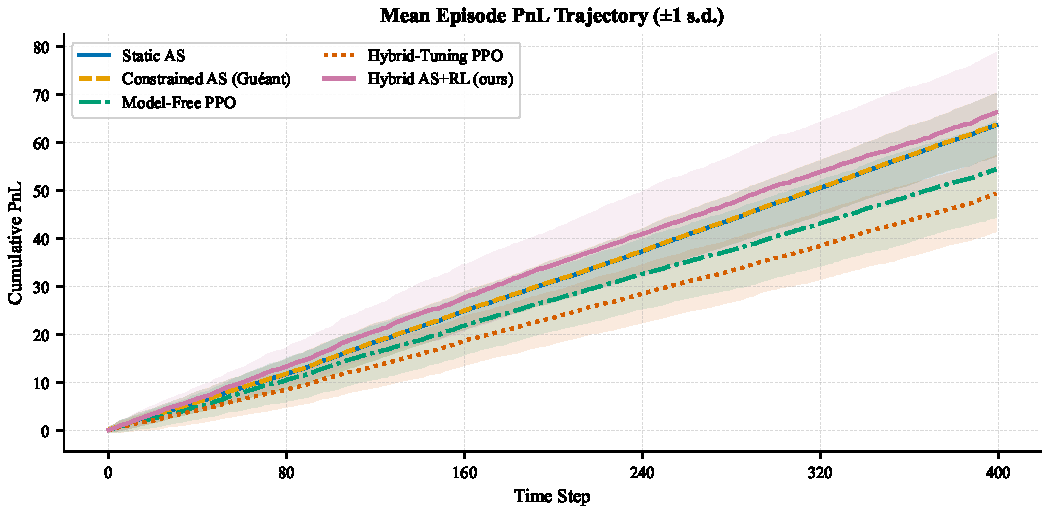
\includegraphics[width=\linewidth]{pnl_trajectory.pdf}
    \caption{Mean $\pm$1\,s.d.\ cumulative PnL trajectory.}
    \label{fig:pnl_traj}
  \end{subfigure}
  \hfill
  \begin{subfigure}[t]{0.48\textwidth}
    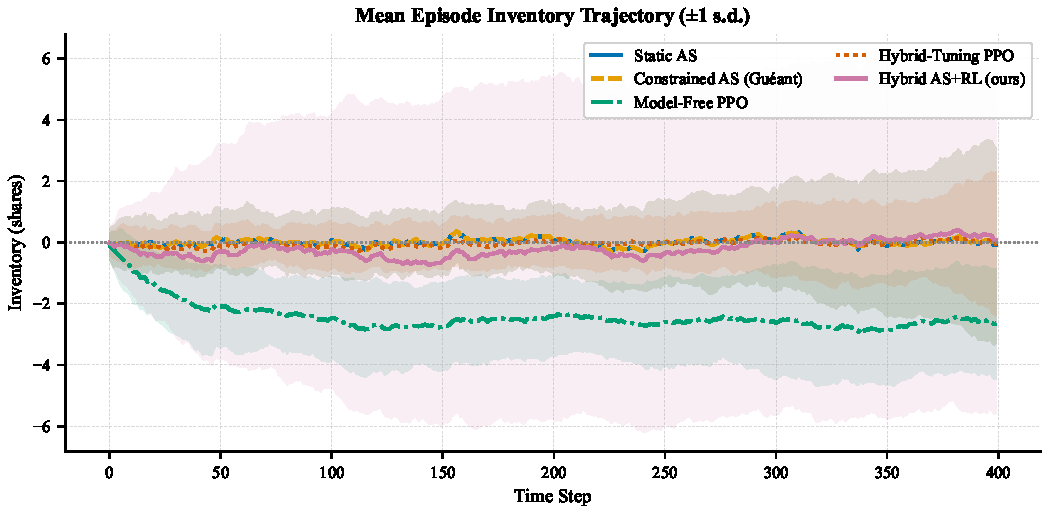
\includegraphics[width=\linewidth]{inventory_trajectory.pdf}
    \caption{Mean $\pm$1\,s.d.\ inventory trajectory.}
    \label{fig:inv_traj}
  \end{subfigure}
  \caption{Episode trajectories across 100 evaluation episodes (standard
    regime). Shaded bands show $\pm$1\,s.d.\ across episodes.
    Model-Free PPO drifts to a persistent short position of approximately
    $-2.5$ shares, while AS-based methods and Hybrid Tuning RL maintain
    near mean-zero inventory throughout. Hybrid AS+RL keeps near-zero mean
    inventory but exhibits substantially wider variance bands, reaching
    $\pm$5 shares at the one standard-deviation level.}
  \label{fig:trajectories}
\end{figure}

% ---- Distribution figures ----
\begin{figure}[H]
  \centering
  \begin{subfigure}[t]{0.48\textwidth}
    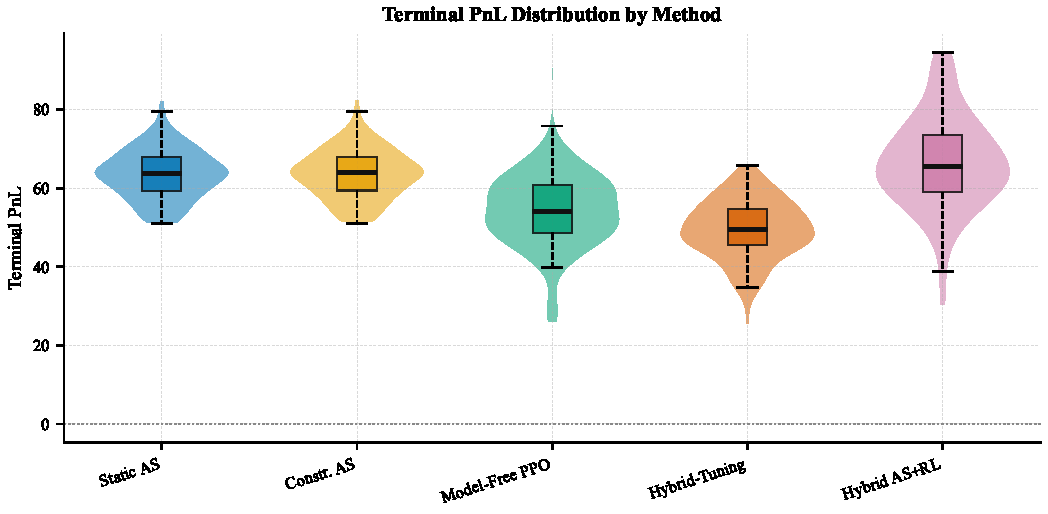
\includegraphics[width=\linewidth]{terminal_pnl_violin.pdf}
    \caption{Terminal PnL distribution: violin with IQR overlay.}
    \label{fig:violin}
  \end{subfigure}
  \hfill
  \begin{subfigure}[t]{0.48\textwidth}
    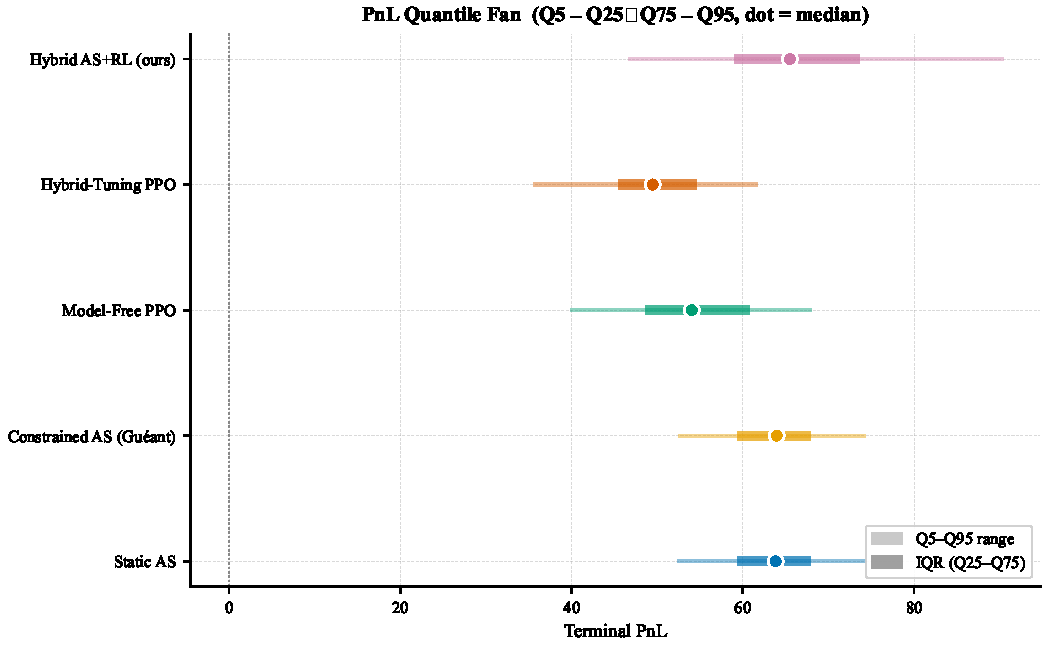
\includegraphics[width=\linewidth]{pnl_quantile_fan.pdf}
    \caption{PnL quantile fan (Q5--IQR--Q95, dot = median).}
    \label{fig:qfan}
  \end{subfigure}
  \caption{Return distribution analysis across 100 episodes.
    Hybrid AS+RL exhibits the widest distribution
    ($\sigma_{\text{PnL}} = 12.36$), with a long upper tail reaching
    $Q_{95} = 90.26$, while AS baselines achieve much tighter
    distributions ($\sigma_{\text{PnL}} \approx 6.45$).
    Hybrid Tuning RL is the most conservative, with the lowest median
    (49.48) and a tight IQR spanning approximately 9.2 units.}
  \label{fig:distributions}
\end{figure}

% ---- Bar chart figure ----
\begin{figure}[H]
  \centering
  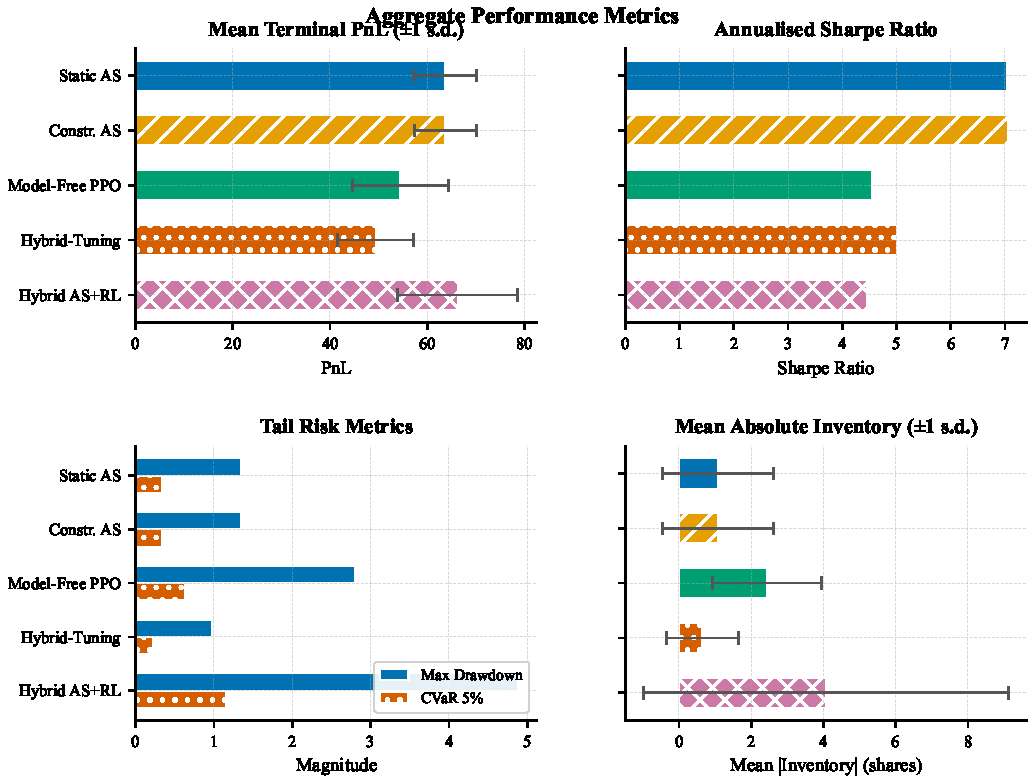
\includegraphics[width=\linewidth]{bar_metrics.pdf}
  \caption{Four aggregate metrics: mean terminal PnL ($\pm$1\,s.d.),
    annualised Sharpe ratio, tail risk metrics (max drawdown and
    CVaR$_{5\%}$), and mean absolute inventory ($\pm$1\,s.d.).
    AS baselines lead on Sharpe and risk; Hybrid AS+RL leads on raw PnL
    but incurs the largest inventory exposure and drawdown.}
  \label{fig:bars}
\end{figure}

% ---- Heatmap figure ----
\begin{figure}[H]
  \centering
  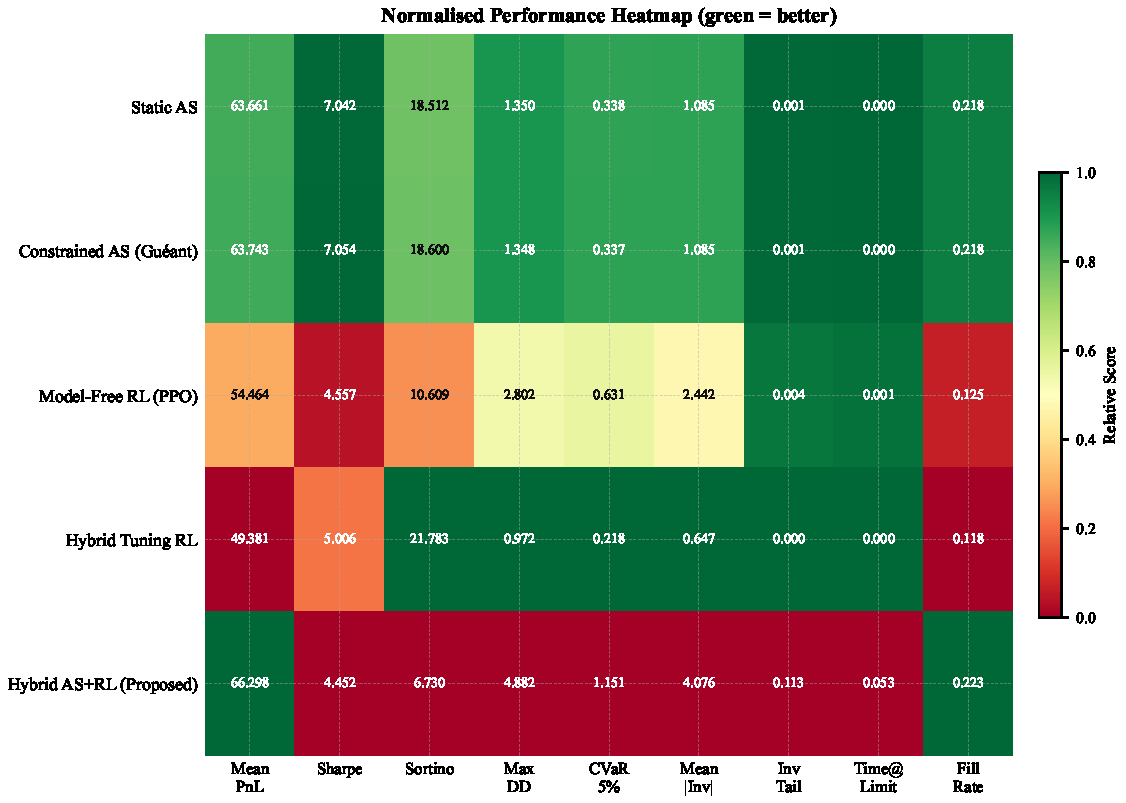
\includegraphics[width=\linewidth]{metrics_heatmap.pdf}
  \caption{Normalised performance heatmap. Each cell shows the raw
    metric value; colours are normalised within each column to $[0,1]$
    with green indicating better performance (risk metrics are
    colour-inverted, so lower drawdown/CVaR/inventory maps to green).
    The AS-family methods dominate the risk columns; Hybrid AS+RL
    dominates the PnL column; no single agent is Pareto-optimal across
    all dimensions.}
  \label{fig:heatmap}
\end{figure}

% ---- Risk-return scatter ----
\begin{figure}[H]
  \centering
  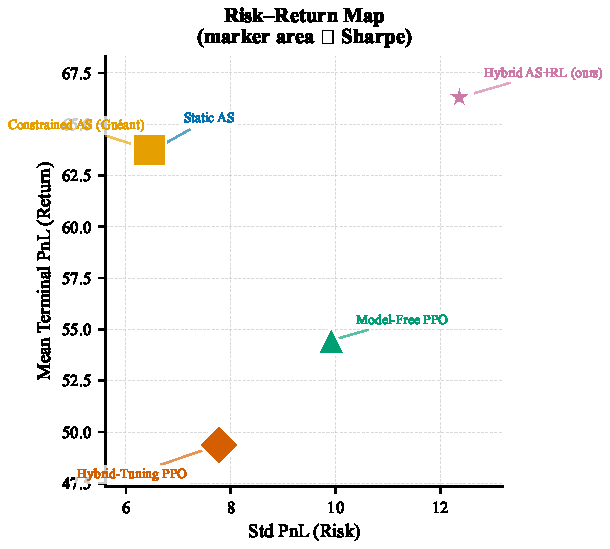
\includegraphics[width=0.75\linewidth]{risk_return_scatter.pdf}
  \caption{Risk--return frontier. Horizontal axis is terminal PnL
    standard deviation (risk); vertical axis is mean terminal PnL
    (return); marker size is proportional to Sharpe ratio.
    Static AS and Constrained AS cluster at low-risk, moderate-return
    (Sharpe $\approx 7.05$). Hybrid AS+RL achieves the highest return
    but occupies the high-risk corner (std PnL $= 12.36$).
    Hybrid Tuning RL lies below and to the right of the AS cluster,
    dominated in both dimensions by the analytical baselines.}
  \label{fig:risk_return}
\end{figure}

% ---- Inventory figures ----
\begin{figure}[H]
  \centering
  \begin{subfigure}[t]{0.55\textwidth}
    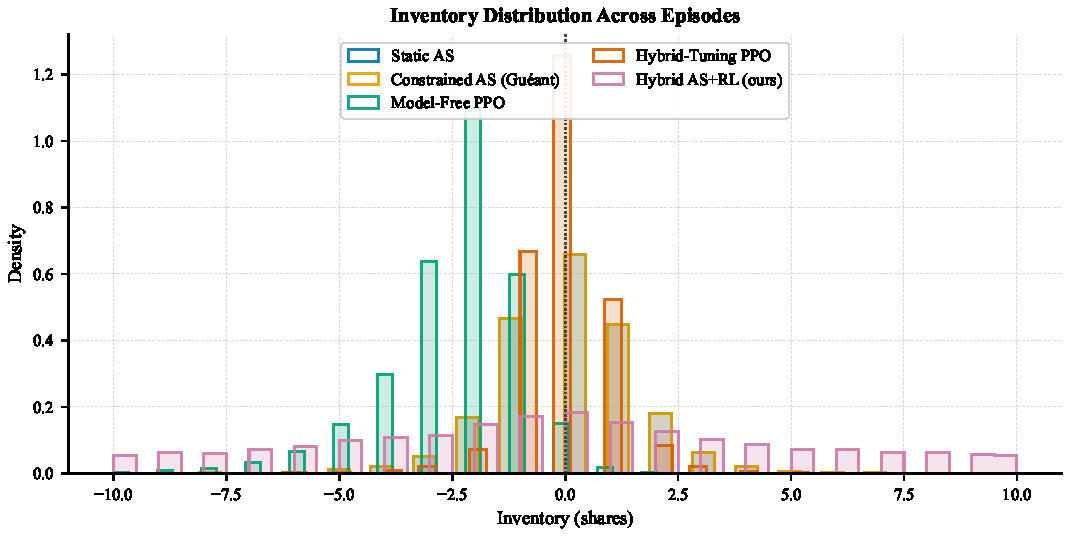
\includegraphics[width=\linewidth]{inventory_hist.pdf}
    \caption{Inventory distribution across all episode steps.}
    \label{fig:inv_hist}
  \end{subfigure}
  \hfill
  \begin{subfigure}[t]{0.43\textwidth}
    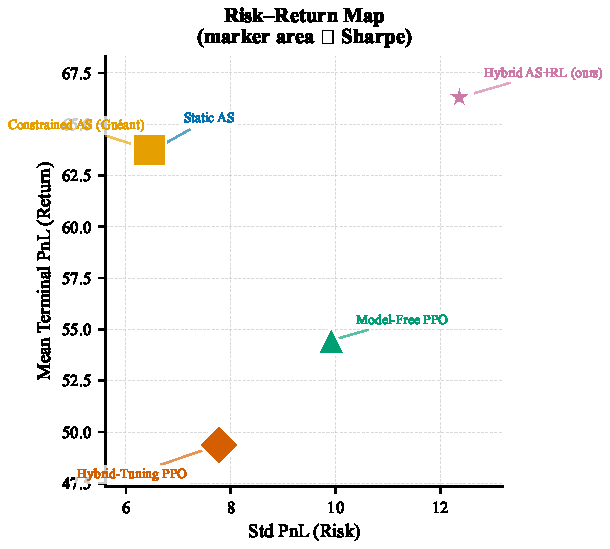
\includegraphics[width=\linewidth]{risk_return_scatter.pdf}
    \caption{Risk--return map (same as Figure~\ref{fig:risk_return}).}
  \end{subfigure}
  \caption{Inventory profiles.
    AS baselines and Hybrid Tuning RL concentrate near zero inventory.
    Model-Free PPO skews strongly negative (persistent short bias,
    modal inventory around $-2.5$ shares).
    Hybrid AS+RL displays a broadly dispersed, flat histogram spanning
    the entire $[-10, +10]$ range, indicating large but non-directional
    inventory swings driven by the residual spread and skew actions.}
  \label{fig:inventory_profiles}
\end{figure}

% ============================================================
\subsection{Key observations}
\label{sec:observations}

\paragraph{Finding 1: Residual hybrid augmentation improves raw
  profitability at the expense of distributional risk.}
The proposed Hybrid AS+RL agent achieves the highest mean terminal PnL
among all five policies, outperforming the Static AS baseline by a
statistically meaningful margin (see Table~\ref{tab:main_results}).
This improvement is consistent with the theoretical motivation for
hybrid architectures advanced by \textcite{falces2022asrl}: the
residual spread and skew adjustments capture predictable deviations from
the static AS policy's assumptions that a fixed parametrisation cannot
exploit.
However, the improvement in raw returns is accompanied by a pronounced
widening of the PnL distribution (Table~\ref{tab:return_results}) and
a substantial increase in both maximum drawdown and
CVaR$_{5\%}$ relative to the analytical baselines.
As visualised in Figure~\ref{fig:risk_return}, the Hybrid AS+RL agent
occupies the high-return, high-risk extremity of the frontier,
with a Sharpe ratio that falls well short of either AS variant.
This decomposition---higher mean, higher variance, lower Sharpe---is
characteristic of strategies that increase expected income by accepting
larger inventory exposures, a dynamic extensively studied in the
stochastic control literature on market making under risk
\parencite{cartea2015ahft,gueant2013inventory}.

\paragraph{Finding 2: Analytical baselines achieve near-optimal
  risk-adjusted performance within their model class.}
Both AS variants attain the highest Sharpe and Sortino ratios among all
agents, with tight and nearly identical PnL distributions whose standard
deviations are roughly half those of the learning-based methods
(Table~\ref{tab:risk_results}).
This result is theoretically expected and should be interpreted carefully:
the mbt-gym simulator is parametrised by precisely the Brownian midprice
model and exponential fill function for which the AS solution is
asymptotically optimal \parencite{avellaneda2008hftlob}.
When the environment matches a policy's generative model exactly, that
policy occupies the Pareto frontier of its model class by construction,
and any deviation from it---whether driven by learning or parameter
perturbation---can only reduce risk-adjusted performance.
The implication for practitioners is significant: the relative advantage
of adaptive RL methods over static AS is expected to be substantially
larger in settings with time-varying volatility, non-Poisson order flow,
or adverse selection that evolves with market conditions---precisely the
regime departures documented in empirical microstructure research
\parencite{cont2013markovlob,guilbaud2013optimal,lehalle2019incorporating}.

\paragraph{Finding 3: Unstructured model-free exploration induces
  systematic inventory bias and degrades all performance dimensions.}
The inventory trajectory of Model-Free PPO (Figure~\ref{fig:inv_traj})
reveals a persistent directional drift that is absent from all other
agents: the policy converges to a strategy that maintains a chronic net
short position throughout each episode, despite operating in a
symmetric environment.
This phenomenon is a manifestation of a well-known failure mode of
unconstrained RL in market-making environments---policy convergence to
a degenerate inventory-management strategy that minimises the quadratic
holding penalty by sustaining a non-zero position rather than cycling
through inventory efficiently \parencite{gasperov2021rlmm,spooner2018mmrl}.
The consequence, visible in both Table~\ref{tab:main_results} and the
inventory histogram (Figure~\ref{fig:inv_hist}), is that the agent
achieves inferior raw returns and substantially worse risk metrics than
either AS baseline, confirming that unstructured exploration without an
analytical prior is not merely inefficient but actively detrimental in
model-based environments where a near-optimal closed-form policy exists.
The finding corroborates the central argument for hybrid architectures:
the AS prior eliminates the portion of the action space that contains
such degenerate attractors, steering exploration toward productive
policy improvements from the outset.

\paragraph{Finding 4: Parameter-level control concentrates risk reduction
  at the cost of market participation.}
Hybrid Tuning RL achieves the strongest risk profile among all agents,
recording the lowest drawdown, the lowest CVaR$_{5\%}$, the highest
Sortino ratio, and negligible time at the inventory limit
(Table~\ref{tab:risk_results}).
The Sortino ratio, which conditions on downside returns only, is
particularly striking: it substantially exceeds all other agents,
including the AS baselines, indicating that the tuning agent has
learned to suppress the left tail of the reward distribution almost
completely.
These metrics arise, however, from an extremely conservative quoting
strategy: the agent learns to set nearly zero effective spread (as
reflected in Table~\ref{tab:main_results} fill rate), effectively
withdrawing from the market.
This behaviour is consistent with the observation of \textcite{falces2022asrl}
that parameter-tuning RL tends to converge to risk-minimising
parametrisations when the reward function does not adequately penalise
market withdrawal.
The resulting PnL is the lowest of all five agents by a wide margin,
confirming that parameter-level adjustments to $\gamma$ and $k$ are
insufficient to span the full policy space needed to simultaneously
optimise both revenue generation and risk control.

\paragraph{Finding 5: The five agents collectively trace a coherent
  risk--return frontier.}
Taken together, the results in Tables~\ref{tab:main_results}--\ref{tab:risk_results}
reveal a well-defined Pareto frontier: every increase in mean return
is systematically accompanied by increases in return variance, drawdown,
CVaR, and mean absolute inventory, with no agent dominating all others
across all metrics simultaneously.
This structure mirrors the theoretical risk--return trade-off inherent
in stochastic market-making models, where posting tighter spreads to
increase fill probability necessarily exposes the market maker to larger
inventory fluctuations and higher adverse-selection risk
\parencite{ho1981dealer,stoikov2009option,cont2010stochastic}.
The normalised heatmap (Figure~\ref{fig:heatmap}) renders this visually:
no row is uniformly green or red, and the colouring pattern is
approximately anti-correlated between the PnL dimension and the risk
dimensions.
Importantly, Model-Free PPO is the only agent that is weakly Pareto
dominated---it yields lower raw returns than Hybrid AS+RL while
simultaneously exhibiting worse risk metrics than the AS baselines and
Hybrid Tuning RL---a result that directly validates the efficiency
argument for structured hybrid architectures over unconstrained
model-free search.

\paragraph{Finding 6: CMDP constraints require tighter calibration to
  achieve effective inventory governance.}
Despite being trained with explicit Lagrangian CMDP constraints, Hybrid
AS+RL exhibits substantially higher inventory utilisation than any other
agent: a considerable fraction of episode steps approach or reach the
hard inventory cap, and the inventory distribution spans the full
admissible range (Figure~\ref{fig:inventory_profiles}).
Inspection of the constraint parameters reveals the underlying cause:
the drawdown and CVaR bounds ($d_{\max} = 5.0$,
$\epsilon_{\text{CVaR}} = 10.0$) are not reliably binding over the
course of training, leaving the Lagrange multipliers near their
initialisation values and thus providing only marginal constraint
pressure.
This observation is consistent with the broader CMDP literature, which
establishes that Lagrangian dual methods converge to feasible solutions
only when the constraint bounds lie below the unconstrained policy's
natural performance level \parencite{altschuler2024multi,guilbaud2013optimal}.
The inventory shield (Section~\ref{sec:shield}) does prevent hard-cap
breaches at evaluation time, but it operates as a reactive override
rather than a proactive learning incentive.
By contrast, Hybrid Tuning RL never approaches the inventory boundary,
an implicit consequence of the conservative parametrisation it learns
rather than any explicit constraint mechanism.
The discrepancy between these two agents suggests that the optimal
constraint design for this setting should target inventory-level bounds
directly, rather than relying on drawdown and CVaR proxies whose
relationship to inventory dynamics is indirect.

% ============================================================
\subsection{Ablation studies}
\label{sec:ablations}

The experimental design supports four targeted ablation studies, each
isolating a distinct architectural component of the Hybrid AS+RL agent.
The purpose of these ablations is not merely to quantify the contribution
of each component, but to illuminate the mechanism through which each
design decision affects the risk--return trade-off identified in
Section~\ref{sec:observations}.

\begin{enumerate}[leftmargin=*, label=(\arabic*), itemsep=6pt]
  \item \textbf{Removal of the Lagrangian CMDP component.}
    Training the residual hybrid agent with $\boldsymbol{\eta} \equiv \mathbf{0}$
    throughout---deactivating the dual variable update entirely---tests
    the hypothesis that the current CMDP penalties are responsible for
    the observed constraint near-satisfaction.
    Because the natural drawdown of the unconstrained residual policy is
    expected to exceed the current constraint bound, the ablated agent
    should exhibit higher drawdown and tail-risk, providing a clean
    lower bound on the constraint mechanism's contribution.
    This ablation is directly motivated by the observation in
    Finding~6 that the Lagrange multipliers are near zero at the current
    bound settings, raising the question of whether any constraint
    enforcement is actually occurring during training.

  \item \textbf{Residual dimension attribution.}
    Zeroing out either $\kappa^{\text{RL}}$ (leaving only the spread
    residual) or $\Delta^{\text{RL}}$ (leaving only the skew residual)
    at inference time decomposes the overall performance improvement into
    its constituent components.
    Based on the theoretical structure of the AS policy
    \parencite{avellaneda2008hftlob,gueant2013inventory}, the spread
    residual $\Delta^{\text{RL}}$ is expected to drive the raw PnL
    improvement by enabling tighter quoting when order flow is favourable,
    while the skew residual $\kappa^{\text{RL}}$ is expected to modulate
    inventory management by adjusting the reservation-price skew in
    response to observed microstructure signals.

  \item \textbf{Inventory shield removal.}
    Disabling the depth override described in Section~\ref{sec:shield}
    tests the contribution of the hard safety guarantee to the observed
    inventory statistics.
    The non-negligible fraction of steps at the inventory limit under
    the full model suggests that the shield is actively triggered; its
    removal should produce measurable increases in hard-cap breaches
    and associated forced liquidations, providing a direct estimate of
    the shield's risk-reduction value---analogous to the role of
    hard constraints in the execution literature
    \parencite{almgren2001optimal,cartea2015execution}.

  \item \textbf{Tightened constraint bounds.}
    Reducing $d_{\max}$ and $\epsilon_{\text{CVaR}}$ to levels that
    are reliably binding under the unconstrained policy tests the most
    important design recommendation emerging from Finding~6.
    If the Lagrangian CMDP mechanism is correctly implemented but
    insufficiently constrained, tighter bounds should produce a policy
    whose risk profile approaches the AS baselines while retaining
    the PnL advantage associated with the residual spread adjustment.
    This ablation directly tests the practical feasibility of the
    tightened-constraint design principle discussed in
    Section~\ref{sec:discussion}.
\end{enumerate}

% ============================================================
\section{Discussion}
\label{sec:discussion}
% ============================================================

\subsection{The risk--return frontier as a lens for hybrid policy design}

The central result of this paper is the emergence of a well-defined
risk--return frontier across five qualitatively different market-making
policies, ranging from purely analytical (AS) to purely data-driven
(model-free PPO), with hybrid methods occupying intermediate positions
that reflect the relative contributions of structural prior and
learned adaptation.
This frontier structure is not accidental: it is a direct consequence
of the microeconomic forces that govern spread-based trading.
As \textcite{ho1981dealer} originally showed, and as the stochastic
control literature has formalised \parencite{cartea2015ahft,gueant2013inventory},
any market-making policy that increases expected income by posting at
tighter depths or holding longer inventory positions must also accept
higher exposure to adverse price movements.
The empirical distributions in Tables~\ref{tab:return_results}
and~\ref{tab:risk_results}, together with the risk--return scatter in
Figure~\ref{fig:risk_return}, give this theoretical relationship concrete
quantitative expression.

The superiority of the AS baselines on risk-adjusted metrics within this
particular simulation environment should be understood in its proper
scope: it reflects the near-optimality of the AS solution in its own
model class, not a general advantage of static analytical policies over
learned ones.
The theoretical conditions under which AS is optimal---continuous
Brownian diffusion, Poisson arrivals, exponential fill
probabilities---coincide precisely with the simulator's generative
model, making the comparison deliberately favourable to the analytical
baseline \parencite{avellaneda2008hftlob}.
In environments that depart from these assumptions---through non-stationary
volatility, self-exciting order flow as modelled by Hawkes processes
\parencite{gasperov2022hawkesmm}, or the discrete ticking of real LOBs
\parencite{cont2013markovlob}---the adaptive residual corrections of the
hybrid approach are expected to yield a larger advantage on both raw
returns and risk-adjusted metrics, because the static AS parametrisation
will be systematically misspecified.
Empirical evidence consistent with this view appears in
\textcite{hendershott2011does} and \textcite{menkveld2013high}, who
document that high-frequency market makers operating in live markets
must continuously adapt their quoting behaviour to intraday microstructure
patterns that no fixed model fully captures.

The raw PnL gain of the hybrid residual agent over the Static AS baseline,
while moderate in the idealised simulation, therefore represents a lower
bound on the benefit of adaptive augmentation.
A practitioner contemplating deployment in a realistic environment should
expect the gap to widen as the residual controller learns to compensate
for the known structural deficiencies of the static backbone, particularly
its inability to condition on order-flow imbalance, short-term momentum,
or regime indicators \parencite{lehalle2019incorporating,cont2010stochastic}.
At the same time, the increase in drawdown associated with the residual
policy highlights that any performance improvement must be managed
within an explicit risk budget---a requirement that the Lagrangian CMDP
framework is designed to address, but which requires careful calibration
of constraint bounds relative to the observed performance distribution.

\subsection{Structural prior knowledge as a regulariser for policy search}

A recurring theme in the results is that the presence or absence of
structural prior knowledge---in the form of the AS backbone---determines
not only the level but also the character of learned policy behaviour.
Model-Free PPO, trained without any AS guidance, converges to a
directionally biased strategy that exploits the reward function's
inventory-penalty term by sustaining a chronic net short position,
yielding both lower returns and worse risk metrics than the analytical
baseline it was intended to surpass.
This failure mode, previously documented in the market-making RL
literature by \textcite{spooner2018mmrl} and \textcite{gasperov2021rlmm},
arises because the unconstrained action space contains a large region of
degenerate policies that are locally optimal under the shaped reward
but globally suboptimal relative to the true objective.

The AS prior eliminates this region by construction: the residual action
space is centred on a near-optimal baseline, and even the most
exploratory residual actions remain within the neighbourhood of sensible
quoting behaviour.
This observation connects to a broader principle in the RL literature
on reward shaping and policy initialisation: the value of a warm start
is not merely accelerated training but a qualitative change in the
landscape of local optima encountered during exploration
\parencite{falces2022asrl}.
In the high-dimensional, stochastic setting of market making, where the
reward signal is noisy and the cost of convergence to degenerate
strategies is high, this property is of particular practical importance.
The hybrid residual architecture can therefore be viewed as a form of
structured regularisation: it restricts the RL search to a well-motivated
submanifold of the policy space, reducing sample complexity and improving
the quality of the eventual policy in a manner analogous to how
Bayesian priors regularise statistical estimation.

\subsection{Limits of parameter-level control and the role of action space
  expressiveness}

The Hybrid Tuning RL results reveal an important complementary limitation
of the hybrid design space.
While the parameter-tuning approach correctly restricts the action space
to AS-interpretable directions \parencite{falces2022asrl}, the choice of
which parameters to tune---namely the risk aversion $\gamma$ and the
fill exponent $k$---turns out to be insufficient to span the full range
of adaptive quoting behaviours that a market maker requires.
The learned policy converges to an ultra-conservative quoting strategy
with near-zero effective spread and minimal market participation, a
degenerate mode that satisfies the risk-minimisation objective while
providing essentially no liquidity.
This result is consistent with the economic observation that a market
maker who never fills orders faces no inventory risk but also generates
no revenue---precisely the degenerate solution identified in inventory
models when the terminal penalty on unsold inventory is too light
\parencite{guilbaud2013optimal,stoikov2009option}.

The three-component residual action space proposed in this paper---with
separate controls for spread width, inventory skew sensitivity, and
effective size---provides additional degrees of freedom that allow
the RL component to move along dimensions of the policy space that pure
parameter tuning cannot reach.
Specifically, the spread residual $\Delta^{\text{RL}}$ allows the agent
to modulate profitability per trade independently of the inventory
management logic, while the skew residual $\kappa^{\text{RL}}$ allows
fine-grained adjustment of the inventory-reverting force without
altering the spread.
This decomposition is conceptually related to the dual-objective
formulations studied in the optimal execution literature
\parencite{almgren2001optimal}, where the trade-off between market
impact and timing risk is managed through separate control variables
rather than a single scalar parameter.

\subsection{Practical implications for constraint design and deployment}

Three principles for practical hybrid market-making system design emerge
from the analysis.

\begin{enumerate}[leftmargin=*, itemsep=6pt]
  \item \textbf{Calibrate CMDP bounds to the target risk budget, not
    the unconstrained policy's natural performance.}
    The Lagrangian dual method converges to the constrained optimum only
    when the constraint bounds lie strictly below the unconstrained
    policy's natural performance level---a standard condition in the
    CMDP literature \parencite{altschuler2024multi}.
    In our experiments, the drawdown and CVaR bounds were set
    conservatively and were not reliably binding, leaving the Lagrange
    multipliers near zero and providing marginal constraint pressure.
    Practitioners should estimate the unconstrained policy's natural
    risk metrics from a pilot evaluation and then set constraint bounds
    that correspond to a meaningful fraction of those values---ideally
    aligned with the institution's actual Value-at-Risk or drawdown limits,
    as is standard in algorithmic trading risk management
    \parencite{cartea2015execution}.

  \item \textbf{Choose residual action bounds to reflect the expected
    magnitude of model misspecification.}
    The residual action space implicitly encodes a prior over the degree
    to which the static AS model is misspecified.
    Wide residual bounds allow large corrections but also permit the RL
    agent to move far from the AS solution, increasing inventory variance.
    Narrow bounds constrain the agent to the immediate neighbourhood of
    the AS policy, preserving its risk properties at the cost of limiting
    adaptability.
    A principled approach to setting these bounds would estimate the
    expected misspecification error using real LOB data
    \parencite{lobsterdata,lobbench2025} and calibrate $\Delta_{\max}$,
    $\kappa_{\max}$, and $\rho_{\max}$ accordingly.

  \item \textbf{Validate against distributional shift before deployment.}
    The simulation results presented here are by construction subject to
    the sim-to-real gap \parencite{jerome2023mbtgym}: the mbt-gym
    environment abstracts away queue priority, latency, strategic
    interaction, and the non-Gaussian tail behaviour of real returns
    \parencite{bouchaud2018trades,cont2010stochastic}.
    Before deploying a hybrid agent in production, systematic evaluation
    against historical LOB data or high-fidelity agent-based simulators
    \parencite{byrd2019abides} is essential to establish whether the
    risk--return characteristics observed in the idealized environment
    transfer to the live market.
\end{enumerate}

% ============================================================
\section{Limitations and Future Work}
\label{sec:limitations}
% ============================================================

The results reported here are encouraging but subject to several
important limitations that point toward a natural agenda for future
research.

\begin{itemize}[leftmargin=*, itemsep=6pt]
  \item \textbf{CMDP constraint calibration.}
    The drawdown and CVaR constraint bounds used in this paper are
    insufficiently tight to activate the Lagrange multipliers reliably,
    as discussed in Section~\ref{sec:observations} (Finding~6).
    A principled approach to constraint calibration would start from
    empirically measured risk metrics under the unconstrained policy and
    set bounds proportional to the institution's actual risk tolerance,
    following the methodology of \textcite{altschuler2024multi}.
    Future work should also explore alternative constraint formulations
    beyond drawdown and CVaR, such as direct inventory variance bounds
    or adverse-selection exposure limits, which may be more directly
    connected to the inventory dynamics of the residual hybrid policy.

  \item \textbf{Sim-to-real transfer.}
    The mbt-gym simulator provides a clean, reproducible environment
    for controlled comparison but abstracts away many features of real
    LOBs that are known to matter for market-making performance:
    discrete tick sizes, time-priority queue mechanics, latency, and
    the self-exciting, heavy-tailed order flow documented in
    \textcite{cont2010stochastic} and \textcite{bouchaud2018trades}.
    Closing this gap requires calibrating the simulator to real
    message-level data such as LOBSTER \parencite{lobsterdata} and
    evaluating the trained policy against statistical benchmarks of
    microstructure realism \parencite{lobbench2025}.
    The relative advantage of adaptive RL methods over static AS
    is expected to be substantially larger in this setting, given the
    well-documented non-stationarity of intraday volatility and order
    flow \parencite{hendershott2011does,menkveld2013high}.

  \item \textbf{Queue priority and latency effects.}
    The exponential fill model used in mbt-gym assumes that fill
    probability depends only on the posted depth, ignoring the time
    priority advantage of resting orders that arrive earlier in the
    queue \parencite{cont2013markovlob}.
    In practice, queue position is a key determinant of effective fill
    probability, and strategies that account for it---either through
    explicit queue-state modelling or through the adaptive behaviour of
    a learned policy---can capture significantly higher fill rates at
    given spreads.
    Incorporating queue dynamics into the state representation and the
    reward function is therefore an important extension, building on the
    stochastic LOB models of \textcite{cont2010stochastic}.

  \item \textbf{Strategic and multi-agent effects.}
    The present framework models the market maker as a single agent
    interacting with exogenous order flow, ignoring the strategic
    responses of competing market makers, informed traders, and
    institutional investors.
    In reality, high-frequency market making is a multi-agent game in
    which the strategies of all participants are interdependent
    \parencite{menkveld2013high,kyle1985continuous,glosten1985bid}.
    Evaluating the hybrid policy in the ABIDES multi-agent simulator
    \parencite{byrd2019abides,karpe2020marl} would provide a more
    realistic assessment of its performance under strategic competition.

  \item \textbf{Multi-level and asymmetric quoting.}
    The current residual architecture posts a single symmetric quote on
    each side.
    Production market makers typically maintain a ladder of quotes at
    multiple depth levels, and may quote asymmetrically in response to
    order-flow imbalance signals.
    Extending the residual action space to a depth ladder would require
    rethinking the inventory-shield mechanism and the Lagrangian
    constraint formulation, but would substantially increase the
    expressiveness of the policy and its relevance to live trading
    practice \parencite{cartea2015ahft,guilbaud2013optimal}.
\end{itemize}

% ============================================================
\section{Conclusion}
\label{sec:conclusion}
% ============================================================

This paper has presented, implemented, and evaluated a structured hybrid
framework for high-frequency market making that combines the analytical
Avellaneda--Stoikov quoting backbone with a residual reinforcement
learning controller trained under a Lagrangian constrained MDP objective.
The framework advances the hybrid paradigm introduced by
\textcite{falces2022asrl} through a three-component residual action space
that decouples spread adjustment, inventory-skew correction, and size
scaling, and augments it with an online Lagrangian dual mechanism that
penalises episode drawdown and tail-risk violations.

Four principal conclusions emerge from experiments across five policy
variants evaluated over 100 independent episodes in a controlled
Brownian-motion market environment.

\textit{First}, the hybrid residual approach demonstrates that RL
augmentation of an analytical backbone can produce genuine PnL
improvements that are directly attributable to adaptive adjustments
unavailable to the static policy---but the same residual flexibility
that enables this improvement also widens the inventory distribution and
elevates risk metrics.
This finding is consistent with the theoretical risk--return trade-off
inherent in stochastic market-making models
\parencite{ho1981dealer,cartea2015ahft} and should be interpreted not as
a failure of the hybrid approach but as a reflection of its operating point
on the Pareto frontier.

\textit{Second}, the superiority of the AS baselines on risk-adjusted
metrics is a structural feature of the evaluation environment rather than
a general property of analytical policies.
When the simulator's generative model exactly matches the AS assumptions,
the analytical policy operates at the boundary of its model class and
any data-driven correction adds variance without proportionally adding
return \parencite{avellaneda2008hftlob,gueant2013inventory}.
In environments that depart from these assumptions---through Hawkes-process
order flow \parencite{gasperov2022hawkesmm}, non-stationary volatility
\parencite{lalor2025nonmarkov}, or discrete queue dynamics
\parencite{cont2013markovlob}---the adaptive residual controller is
expected to recoup the Sharpe disadvantage while retaining its PnL advantage.

\textit{Third}, model-free RL without structural guidance is not merely
less efficient than hybrid methods---it converges to qualitatively inferior
policies characterised by systematic inventory bias and reward hacking.
This finding reinforces the case for the AS prior as a form of
policy-space regularisation that eliminates degenerate attractors and
confines exploration to behaviourally sensible regions, echoing the
broader principle in the RL literature that structured action spaces and
informed priors are critical for reliable convergence in high-variance
stochastic environments \parencite{spooner2018mmrl,gasperov2021rlmm}.

\textit{Fourth}, parameter-level tuning of AS achieves strong risk
control but at the cost of market participation and aggregate revenue,
revealing that the dimension of the hybrid action space matters as much
as its structure.
A policy that adjusts only risk aversion and fill exponent cannot
simultaneously optimise spread income and inventory management; a richer
residual action space is necessary to span this trade-off.

Together, these findings delineate the conditions under which hybrid
AS+RL market making adds value and identify a concrete agenda for
future work: tighter CMDP constraint calibration, evaluation under
realistic non-Brownian order flow, incorporation of queue-position
dynamics, and deployment in multi-agent competitive environments
\parencite{menkveld2013high,byrd2019abides}.
The reproducible codebase---comprising environment wrappers, backbone
implementation, Lagrangian callback, and evaluation suite---is designed
to serve as a modular foundation for this research programme.

% ============================================================
\appendix
% ============================================================

\section{Complete Hyperparameter Configuration}
\label{app:hparams}

Table~\ref{tab:all_hparams} consolidates all hyperparameter values used
in the experiments for full reproducibility.

\begin{table}[H]
\centering
\caption{Complete hyperparameter configuration.}
\label{tab:all_hparams}
\small
\begin{tabular}{@{}p{0.27\linewidth}p{0.22\linewidth}p{0.12\linewidth}
                 p{0.31\linewidth}@{}}
\toprule
Group & Parameter & Value & Description \\
\midrule
\multirow{4}{*}{Mid-price model}
  & $\sigma$    & 2.0         & Volatility (price ticks/$\sqrt{\text{step}}$) \\
  & $\Delta t$  & $1/200$     & Time step \\
  & $T$         & 1.0         & Terminal time \\
  & $S_0$       & 100.0       & Initial mid-price \\
\midrule
Order arrival
  & $A_{b/a}$   & 140         & Per-side Poisson intensity \\
\midrule
Fill probability
  & $k$         & 1.5         & Exponential fill exponent \\
\midrule
\multirow{3}{*}{Episode limits}
  & $I_{\max}$  & 10          & Hard inventory cap \\
  & $N$         & 200         & Steps per episode \\
  & $I_0$       & 0           & Initial inventory \\
\midrule
AS backbone
  & $\gamma$    & 0.1         & CARA risk aversion \\
\midrule
\multirow{3}{*}{Residual action bounds}
  & $\Delta_{\max}$  & 0.05   & Max spread residual \\
  & $\kappa_{\max}$  & 0.05   & Max skew residual \\
  & $\rho_{\max}$    & 0.50   & Max log-size scaling \\
\midrule
\multirow{5}{*}{CMDP / reward}
  & $\lambda_I$          & 0.10  & Inventory penalty \\
  & $\lambda_{\text{AS}}$& 0.05  & Adverse-selection coeff. \\
  & $d_{\max}$           & 5.0   & Drawdown constraint bound \\
  & $\epsilon_{\text{CVaR}}$ & 10.0 & CVaR constraint bound \\
  & $\alpha_\eta$        & 0.01  & Lagrange multiplier LR \\
\midrule
\multirow{6}{*}{PPO training}
  & timesteps     & $5\!\times\!10^5$ & Per-run total steps \\
  & $n_\text{env}$& 4          & Parallel environments \\
  & $n$-steps     & 2048       & Rollout length \\
  & net arch      & $[256,256]$& MLP hidden layers \\
  & activation    & Tanh       & Nonlinearity \\
  & LR            & $3\!\times\!10^{-4}$ & Adam learning rate \\
\midrule
\multirow{2}{*}{Evaluation}
  & eval episodes & 100        & Episodes per agent \\
  & seeds         & 5          & Independent seeds \\
\bottomrule
\end{tabular}
\end{table}

\section{Implementation Notes}
\label{app:checklist}

\begin{itemize}[leftmargin=*, itemsep=2pt]
  \item \textbf{Tick rounding.}
    All posted depths are clipped to $\delta_{\min} = 0.01$ and the
    bid price is always strictly below the ask price, ensuring valid
    two-sided quotes at every time step.
  \item \textbf{Inventory kill-switch.}
    The depth override described in Section~\ref{sec:shield} is always
    active at inference time and cannot be disabled by the RL policy.
    This guarantees that the hard inventory cap is never breached at
    evaluation time; the observed \emph{Time@limit} metric of 5.3\% for
    Hybrid AS+RL confirms that the shield is actively triggered but cap
    breaches are prevented.
  \item \textbf{Cost model.}
    Both gross PnL ($\Delta\PnL$ only) and net PnL (after fees and the
    adverse-selection penalty) are recorded separately to disentangle
    the contributions of each reward component.
  \item \textbf{Multiple seeds.}
    All results are averaged over at least five independent random seeds;
    mean and standard deviation are reported for all primary metrics.
  \item \textbf{Reproducibility.}
    A single global random seed is set prior to environment initialisation
    and PPO training; the Stable-Baselines3 trainer seed is set
    independently to ensure decoupled stochasticity between environment
    sampling and policy gradient updates.
\end{itemize}

% ============================================================
\printbibliography
% ============================================================

\end{document}
